\documentclass[pdflatex,sn-mathphys]{sn-jnl} % Springer Nature template for NCA

%------------------------------------------------------------------------------
% PACKAGES
%---------------------------------------------------------------------------

\usepackage[normalem]{ulem}

\usepackage{amsmath,amssymb,amsfonts}
\usepackage{graphicx}
\usepackage{booktabs}
\usepackage{float}
\usepackage{subcaption}
\usepackage{caption}
\usepackage[table]{xcolor}
\usepackage{hyperref}
\hypersetup{colorlinks=true, allcolors=blue}
\usepackage{textcomp}
\usepackage[numbers]{natbib}
\usepackage{rotating}
\raggedbottom

%------------------------------------------------------------------------------
% BEGIN DOCUMENT
%------------------------------------------------------------------------------
\begin{document}

%------------------------------------------------------------------------------
% ABSTRACT
%------------------------------------------------------------------------------
\vspace{1em}
\section*{Abstract}
\noindent
Accurate crop classification from satellite imagery is essential for agricultural monitoring, yield forecasting, and food security assessment, yet remains particularly challenging in dryland farming regions of the Global South where spectral similarity between crop types, irregular phenological cycles, and persistent cloud cover complicate classification. We address this gap using a uniquely rich labeled field-boundary dataset from the Western Cape of South Africa to conduct a systematic comparison of machine learning, deep learning, and patch-based approaches under conditions of high environmental heterogeneity. Classical models — including XGBoost, Random Forest, and LightGBM — were enhanced with automated time-series feature extraction via \texttt{xr\_fresh}, which has not previously been evaluated in the crop classification literature. We benchmarked these against deep learning architectures that learn directly from raw multi-temporal Sentinel-2 pixel sequences, including a CNN-BiLSTM hybrid, a TabNet ensemble, and a 3D CNN ensemble applied at the patch level. Our results show that a field-level voting classifier achieved competitive performance (Kappa 0.69, F1 0.76) with substantially lower computational cost, while the CNN-BiLSTM ensemble achieved the highest field-level performance overall (Kappa 0.77, F1 0.84), surpassing the best classical approach by approximately 0.08 in both metrics without relying on hand-crafted features. Patch-based 3D CNN models contributed additional spatial context but did not exceed pixel-level deep learning performance. These findings demonstrate that end-to-end sequence modeling can outperform automated feature engineering in complex agricultural landscapes, while classical approaches remain viable in resource-constrained operational settings.


\vspace{1em}
\noindent\textbf{Keywords:} Crop classification, Satellite imagery, Deep learning, Machine learning, Remote sensing

\section{Introduction}

Accurate and timely crop classification is foundational to precision agriculture, enabling yield forecasting, resource optimization, food security assessment, and climate-resilient decision-making \cite{sciencedirect2023, ieee2017}. The widespread availability of high-resolution Earth observation data, especially from the Sentinel-2 satellite constellation, has transformed the landscape of agricultural monitoring. With 13 spectral bands, spatial resolutions ranging from 10 to 60 meters, and a revisit frequency of approximately five days, Sentinel-2 offers dense multi-temporal imagery rich in spatial and spectral information.

Despite these advancements, reliable crop classification remains a complex task on plots throughout Africa and the Global South. Spectral similarities between crops, temporal variability in planting and phenological cycles, and atmospheric disturbances such as cloud cover hinder classification accuracy. In Africa, this is compounded by the complexities of rain-fed dryland farming \cite{begue2020}. Traditional machine learning methods often rely heavily on manually engineered features, such as vegetation indices or statistical summaries, which may capture pertinent temporal and spectral dynamics but are often more limited in complexity of features. A number of methods like XGBoost (XGB) and Random Forest (RF) have proven effective in a variety of crop mask and classification tasks \cite{mahlayeye2024, mann2017, mann2019}. However in regions with significant differences in cropping patterns and practices, the complexity of the task can outstrip the exploitable variability in the training data \cite{mann2025, mahlayeye2024}. Newly released automated feature extraction methods like that implemented in xr\_fresh offer the possibility of rich feature sets for use in machine learning but it remains untested in the literature \cite{mann2025}. Despite their effectiveness, machine learning methods can be inconsistent \cite{feyisa2020}. Several factors contribute to this variability, including hyperparameter selection \cite{saini2018}, sample quality and quantity \cite{jin2019}, selection of training and testing splits \cite{belgiu2016}, imbalanced classes \cite{belgiu2016}, and feature generation and selection \cite{penabarragan2011}.  

To address these limitations, deep learning approaches have gained traction in crop type mapping, with both Recurrent Neural Networks (RNNs) and Convolutional Neural Networks (CNNs) emerging as particularly promising architectures. RNNs are well suited to the sequential nature of remote sensing time series, as their internal hidden states allow them to retain a form of memory across time steps, capturing the temporal dynamics of crop phenology that static or summary-based features often miss. This capacity to model temporal structure has proven especially valuable for crop classification in data-rich environments, where the full growing season trajectory of spectral signals can be exploited \cite{teixeira2023, zhu2017}. The lack of high quality training data in the Global South and lack of reliable cloud-free imagery has pushed many of the most successful efforts into the realm of precision agriculture such as applications for hyperspectral and drone-derived imagery \cite{mahlayeye2024}. Nevertheless, recent work applying deep learning to agricultural mapping in developing world contexts has demonstrated encouraging results. Ayushi et al. \cite{buttar2024} applied a U-Net fully convolutional encoder-decoder architecture to a crop type mapping task in Kenya, and Liu et al. \cite{liu2024} used a convolutional neural network (3D-CNN) both achieving F1 scores over 73\%. However questions remain about the generalizability of deep learning models particularly in complex environments with limited training data \cite{pankajakshan2026}. 

Hybrid approaches offer a compelling opportunity by combining the representational power of deep learning with the interpretability and efficiency of traditional machine learning, and several studies have demonstrated their value in agricultural remote sensing contexts. A common strategy in precision agriculture involves using a pre-trained deep learning model as a feature extractor especially, with the resulting high-level representations passed to a traditional classifier for the final prediction. Espejo-Garcia et al. \cite{espejo2020} fine-tuned architectures including MobileNet, DenseNet, and Xception before replacing their fully connected layers with Support Vector Machines and Gradient Boosting classifiers for weed identification, while Koklu et al. \cite{koklu2022} found that pairing MobileNetV2 feature extraction with an SVM consistently outperformed end-to-end deep learning for grapevine leaf classification. Yang et al. \cite{yang2020} more relevant to this study, combined a CNN with a Random Forest classifier for Sentinel-2 crop type mapping, leveraging the spatial-spectral learning capacity of the CNN alongside the robustness and resistance to overfitting characteristic of ensemble tree methods. Of particular relevance to data-scarce environments, Nowakowski et al. \cite{nowakowski2021} demonstrated that integrating transfer learning with traditional machine learning algorithms achieved high classification accuracy in Malawi, suggesting that hybrid architectures may be especially well suited to the constraints of the Global South. Taken together, these hybrid approaches suggest a productive middle path between the interpretability and data efficiency of classical machine learning and the feature-learning capacity of deep neural networks, and they form part of the methodological landscape against which the approach taken in this study is positioned.
 
This study addresses a critical yet underexplored gap in the crop classification literature: the systematic comparison of machine learning, deep learning, and hybrid approaches under the constraints typical of the Global South, but with the advantage of an unusually rich, high-quality training dataset. While much of the methodological literature has been developed and validated in data-rich temperate agricultural settings, the Western Cape of South Africa presents a distinct set of challenges — smaller field sizes, rain-fed dryland farming systems, heterogeneous and spatially variable planting rotations, persistent cloud cover during the critical winter growing season, and phenological cycles that do not conform to the assumptions embedded in many widely used models.  We leverage this rare combination of environmental complexity and labeled data richness to conduct a rigorous evaluation of methods that are seldom compared within a single study and region. Our experiments utilize a labeled field-boundary dataset provided by Radiant Earth's MLHub \cite{mlhub}, capturing ground-truth crop types for agricultural fields in South Africa during the 2017 growing season. 

We propose and evaluate multiple deep learning architectures — including CNN-BiLSTM hybrids, TabNet Classifier ensembles, and 3D CNN models — that extract dynamic phenological features across time, and benchmark these against traditional ensemble methods including XGBoost and Random Forest. A key novelty of this study is the evaluation of \texttt{xr\_fresh}, an automated time-series feature extraction framework that has not previously been tested in the crop classification literature, both as a standalone input to classical classifiers and as a component of hybrid pipelines that combine automated feature richness with deep learned representations. Throughout, we restrict our inputs to multi-temporal Sentinel-2 optical imagery alone, without recourse to SAR data, in order to isolate the signal available from spectral time series and maximize applicability to contexts where only optical data is available. All code is publicly available to support reproducibility and future research \cite{capstone_repo}. 

This leads to the central research question: across a range of machine learning, deep learning, and hybrid architectures, which approach most reliably classifies crop types from multi-temporal Sentinel-2 optical imagery in a complex dry-land farming environment, and can hybrid methods and automated feature extraction match or exceed the performance of end-to-end deep learning under conditions of high environmental heterogeneity and limited labeled data?


\subsection{Related Work}

Crop classification using satellite imagery has become a core task in precision agriculture because it supports large-scale crop monitoring, yield estimation, resource management, and food-security analysis. The increasing availability of high-resolution, multi-temporal Earth observation data, particularly from Sentinel-2, has enabled substantial progress in crop mapping, but several challenges remain. These include strong spectral similarity among crop types, temporal variability in planting and phenological cycles, class imbalance, and the difficulty of building methods that generalize across regions and farming systems.

Early work in crop classification relied primarily on classical machine learning methods such as Random Forest, Support Vector Machines, Logistic Regression, and gradient-boosted tree models. These approaches typically operate on hand-crafted inputs derived from spectral bands, vegetation indices, temporal summaries, or other engineered descriptors, and they have often proven effective because they are computationally efficient, interpretable, and robust on structured remote-sensing data \cite{maxwell2019, ieee2017}. However, their performance depends heavily on feature engineering and domain knowledge, which can limit transferability across crop systems and agroecological regions. This challenge becomes especially pronounced in heterogeneous agricultural landscapes, where differences in management practices, field conditions, and phenological timing can reduce the separability captured by manually designed features \cite{maxwell2019, ieee2017}.

These limitations have motivated growing interest in deep learning approaches that learn hierarchical feature representations directly from raw or minimally processed observations. Convolutional neural networks (CNNs) are effective at extracting local spectral and spatial patterns, while recurrent architectures such as LSTMs and BiLSTMs are well suited to modeling temporal crop-development signals over a season. More broadly, deep learning has become increasingly important in remote sensing because it reduces reliance on manually constructed predictors and can capture complex temporal structure that summary statistics often miss \cite{zhu2017, teixeira2023}. Prior work has shown that temporal modeling is especially valuable when crop types are difficult to distinguish from single-date imagery but follow different seasonal trajectories \cite{russwurm2018, wardlow2007towards}.

A particularly important direction in the literature has been the development of hybrid architectures that combine convolutional feature extraction with temporal sequence modeling. For example, Fan et al.\ proposed a hierarchical convolutional recurrent neural network for Sentinel-2 image classification, showing that combining CNN-based feature extraction with recurrent modeling can improve classification robustness relative to both classical and standalone deep learning baselines \cite{fan2023hcrnn}. Similarly, Tufail et al.\ demonstrated that hybrid CNN-RNN models applied to multi-temporal Sentinel-2 imagery and red-edge vegetation indices can achieve very strong crop-mapping performance by jointly learning spatial context and temporal phenology \cite{tufail2025cnnrnn}. Bandar and Co\c{s}kun\c{c}ay likewise showed that combining an attention-based BiLSTM with a temporal CNN improves crop classification from Sentinel-2 time-series data, reinforcing the broader value of spatiotemporal representation learning in agricultural remote sensing \cite{bandar2024bilstm}.

Beyond fully end-to-end deep architectures, several studies have explored hybrid pipelines that combine learned representations with classical machine learning classifiers. Espejo-Garcia et al.\ used deep convolutional backbones as feature extractors before applying conventional classifiers for weed identification, while Koklu et al.\ found that deep features combined with an SVM outperformed end-to-end models for grapevine leaf classification \cite{espejo2020, koklu2022}. In a setting more directly related to this study, Yang et al.\ combined CNN-based representation learning with a Random Forest classifier for multi-temporal crop classification from Sentinel-2 imagery \cite{yang2020}. Transfer-learning-based hybrid approaches have also shown promise in data-constrained environments; for example, Nowakowski et al.\ reported strong crop-type mapping results in Malawi using transfer learning combined with traditional machine learning \cite{nowakowski2021}. Taken together, these studies suggest that hybrid approaches can provide a useful middle ground between the flexibility of deep learning and the robustness and interpretability of classical models.

The representation of input data is another central theme in the literature. Sentinel-2 has become a preferred platform for crop monitoring because of its high revisit rate and multispectral richness, and vegetation indices such as NDVI and EVI are often incorporated to improve crop separability. While such features are informative, they remain manually designed and may not fully capture the complexity of crop development when used in isolation. This has led to increasing interest in either end-to-end models that learn directly from temporal reflectance sequences or automated feature-extraction frameworks that summarize time-series behavior more comprehensively.

Despite these advances, important gaps remain. Much of the crop-classification literature has been developed and validated in relatively data-rich or homogeneous agricultural settings, whereas crop mapping in the Global South often involves additional complications such as rain-fed dryland farming, heterogeneous field conditions, irregular planting calendars, persistent cloud cover, and limited access to dense labeled training data \cite{begue2020,mahlayeye2024}. These conditions make it unclear which modeling strategy is most reliable in operational settings where both environmental complexity and data limitations are substantial.

Our study is positioned within this gap. Rather than evaluating a single architecture in isolation, we conduct a systematic comparison of classical machine learning, deep learning, and patch-based approaches for crop classification using multi-temporal Sentinel-2 imagery in the Western Cape of South Africa. In doing so, we build on prior work in temporal modeling, hybrid learning, and ensemble-based classification, while also evaluating \texttt{xr\_fresh} as an automated time-series feature-extraction framework in a crop-classification setting \cite{mann2025}. This allows us to assess whether automated feature extraction can remain competitive with end-to-end deep sequence models in a complex dryland farming environment.


%\textbf{I THINK THESE SECTIONS ARE ALREADY ADDRESSED IN THE INTRODUCTION OR IS THIS PART OF THE STYLE OF THE MANUSCRIPT??  pLEASE EMAIL ME IF YOU NEED TO INCLUDE IT}

%\subsubsection{Synthesis and Research Gap} 
%While the literature demonstrates strong progress in crop classification using both traditional and deep learning methods, significant gaps remain. Most existing studies are either limited to single crop types, small regions, or heavily reliant on handcrafted features. Few studies rigorously evaluate field-level classification performance using large-scale, multi-temporal Sentinel-2 imagery with minimal feature engineering. Furthermore, the operational scalability and generalization of ensemble deep learning models across diverse agroecological conditions remain under explored. Our work addresses these gaps by proposing a scalable, field-level crop classification framework that integrates deep sequence models with minimal reliance on handcrafted features, benchmarked against both classical and ensemble learning baselines.

%\section{Problem Statement}

%Accurate crop classification using satellite imagery remains a significant challenge due to spectral similarities among crops, temporal variability in growth cycles, and the limitations of traditional models that rely on manually engineered features. In regions like South Africa, where each field polygon typically represents a single crop type, these challenges hinder effective agricultural monitoring and decision-making. This study addresses the critical problem of how to effectively leverage the rich spectral and temporal information provided by multi-temporal Sentinel-2 imagery to classify crop types at the field level with high precision. By focusing on deep learning architectures that do not depend on handcrafted features and by comparing them with classical machine learning baselines, the research aims to overcome existing limitations and contribute a scalable, data-driven solution for accurate crop type identification.


\section{Data Description}

The dataset used for this study consists of two primary components: satellite imagery and field boundary data, as sourced from \cite{sa_comp}.

\subsection{Study Area and Description}

The study was conducted in an agriculturally productive region of South Africa, characterized by diverse agroecological conditions and cropping systems. Major crop types in the dataset include wheat, barley, canola, small grain grazing, and lucerne/medics (alfalfa). The region spans varying climatic zones, from semi-arid to subtropical—and exhibits seasonal differences in rainfall and temperature, contributing to distinct crop phenologies.

Field parcels differ in size, shape, and management practices, introducing heterogeneity into the dataset. Sentinel-2 imagery was collected monthly across the 2017 growing season, covering key phenological stages from emergence to harvest. This temporal resolution is vital for capturing crop-specific growth patterns, which are often indistinguishable in single-date imagery.


\subsection{Remote Sensing Data}

Sentinel-2 Level-2A optical surface-reflectance data were acquired as monthly cloud-free composites over the study area in South Africa for the January–December 2017 growing season. Monthly median composites were generated using a 30\% \texttt{s2cloudless} cloud-probability filter combined with a morphological cloud-shadow mask clipped to field boundaries, scaled to integer reflectance ($\times$10,000), and exported as 10 m single-band GeoTIFFs via Google Earth Engine. From each monthly composite, six informative features were extracted: four optical bands — B2 (Blue, 490 nm), B6 (Red Edge 1, 740 nm), B11 (SWIR 1, 1610 nm), and B12 (SWIR 2, 2190 nm) — alongside the Enhanced Vegetation Index (EVI) and Hue, a colorimetric feature derived from spectral reflectance to characterize vegetation condition \cite{mann2023}. These bands were chosen because they have be used extensively in the literature for agricultural modeling. 

Each feature was captured across 11 temporal observations during the growing season; however, due to persistent cloud cover, data from May and June 2017 were excluded, yielding 10 valid monthly observations per feature. Each pixel was consequently represented by a 60-dimensional time-series feature vector, enabling the capture of rich phenological dynamics across the season.

We acknowledge that computing EVI from monthly median composites may introduce spectral inconsistencies, as the EVI formula assumes band values collected simultaneously. While median compositing is effective for reducing cloud contamination, it may distort the physical interpretation of EVI due to temporal misalignment across bands. This approach was nonetheless adopted as a pragmatic trade-off to maintain temporal continuity across the growing season under frequent cloud cover. As the primary objective was to capture general phenological trends rather than precise instantaneous reflectance values, this method was considered sufficient for downstream classification. Future work may explore pixel-wise temporal filtering or gap-filling strategies that preserve per-date band consistency for vegetation index computation.

By relying exclusively on optical data rather than SAR imagery \cite{sar2022}, this study demonstrates the capability of multi-temporal spectral analysis alone for robust crop classification. This approach is directly transferable to emerging high-resolution optical platforms such as PlanetScope, reinforcing the operational relevance of dense, temporally-aware optical remote sensing for agricultural monitoring at scale.

\subsection{Field Boundary Data}

The field boundary polygons were drawn from the crop type classification dataset for Western Cape, South Africa \cite{mlhub}. This GeoJSON file delineated each agricultural field as a polygon, with boundaries digitized primarily from 50 cm aerial photography at scales of 1:2,500 for horticultural parcels and 1:7,500 for other fields between May and August 2017. In cases where ground reference was unavailable, Sentinel-2 imagery supplemented the digitizing process. Each polygon fully encompassed the field area and carried a crop-type label obtained via aerial and vehicle surveys conducted from May 2017 to March 2018 \cite{mlhub}. 

All predictions in our study were made at the field level.


\subsection{Crop Types and Distribution}

In this study, we classified five crop types: wheat, canola, lucerne/medics (alfalfa), barley, and small-grain grazing.

\begin{figure}[ht]
  \centering
  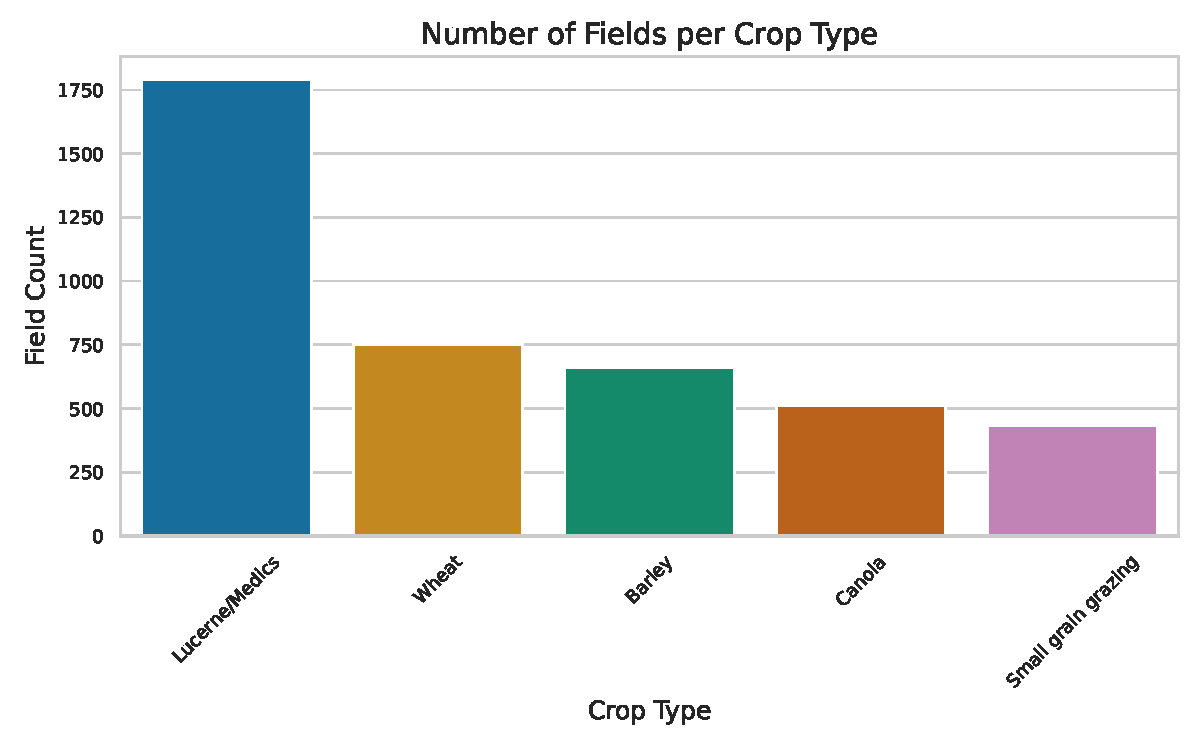
\includegraphics[width=0.55\textwidth]{fields_count.pdf}
  \caption{Number of fields per crop type.}
  \label{fig:EDA-1}
\end{figure}

Figure~\ref{fig:EDA-1} illustrates the distribution of crops in the study area. The data was notably imbalanced, with the majority of fields dedicated to lucerne/medics. The imbalance in crop representation has important implications for model training and evaluation, as classification algorithms may be biased towards the majority class unless appropriate balancing techniques are applied.

\begin{figure}[ht]
  \centering
  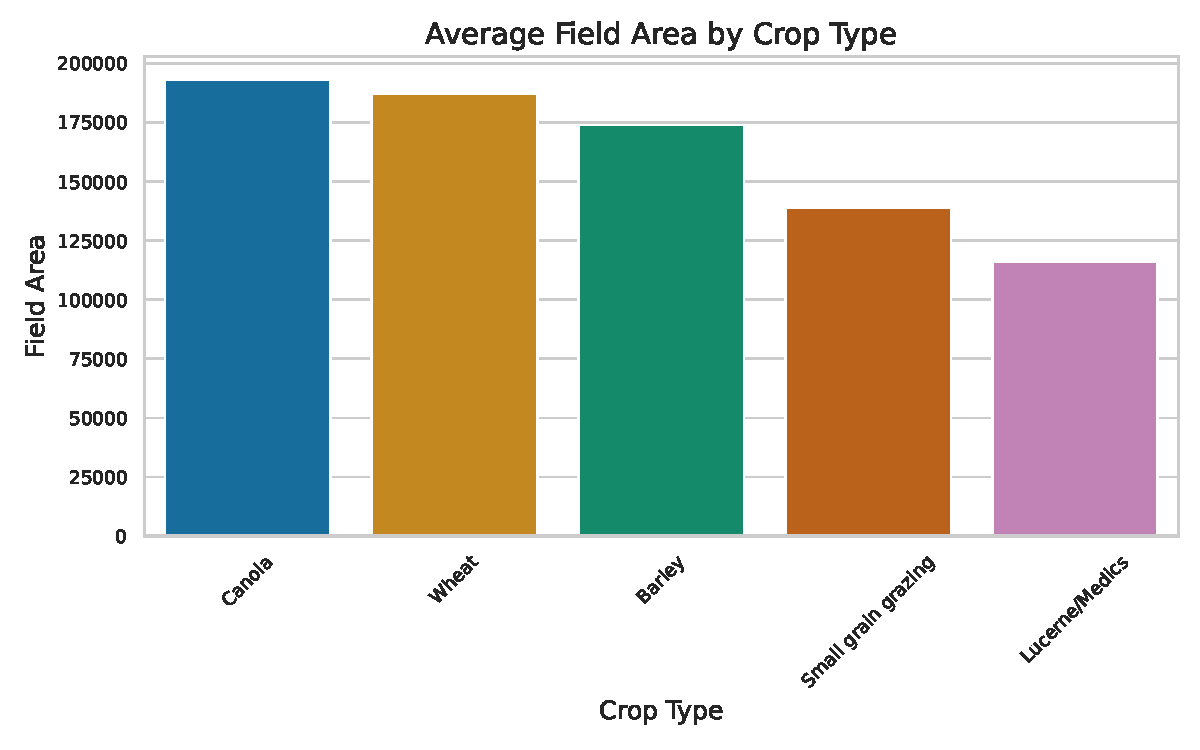
\includegraphics[width=0.55\textwidth]{avg_field_area.pdf}
  \caption{Average field area by crop type.}
  \label{fig:EDA-2}
\end{figure}

Figure~\ref{fig:EDA-2} presents the mean field area for each crop type, measured in square metres (m\textsuperscript{2}). Although lucerne/medics represent the majority of fields, their average area is smaller compared to other crop types.

\begin{figure}[ht]
  \centering
  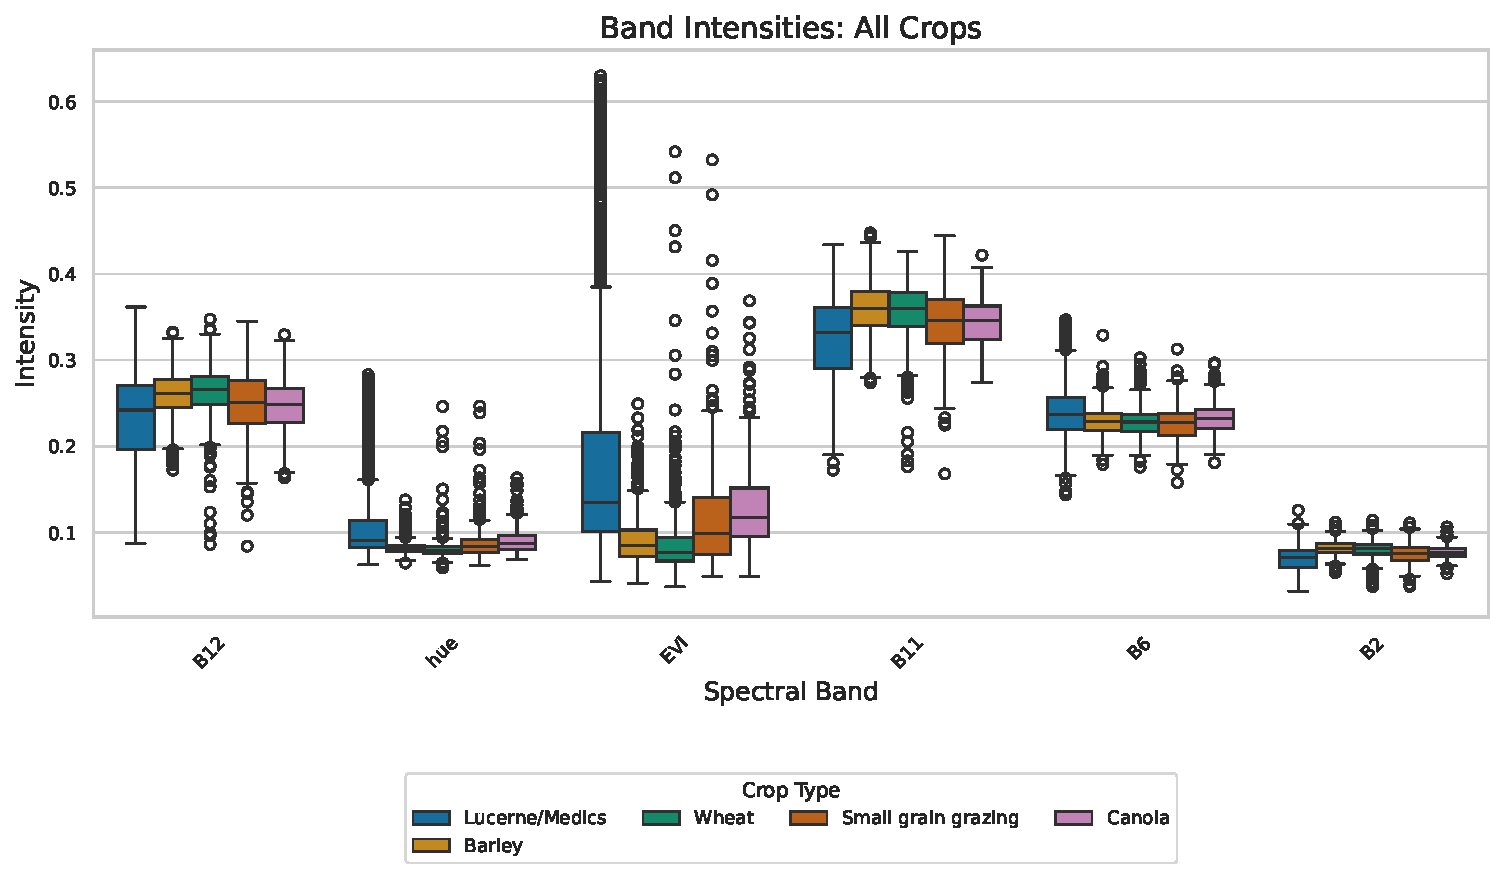
\includegraphics[width=0.55\textwidth]{all_crops_boxplot.pdf}
  \caption{Boxplots of spectral band intensities for each crop type, showing the distribution and overlap of spectral responses.}
  \label{fig:EDA-3}
\end{figure}

Figure~\ref{fig:EDA-3} displays box plots of spectral band intensities for each crop type, illustrating the distribution and overlap of spectral responses. Although some differences in median and spread are evident, the substantial overlap in spectral intensities across crops demonstrates that classification based solely on a limited set of spectral bands is challenging and prone to confusion. This was particularly true for cereal crops such as wheat and barley, which exhibited highly similar spectral profiles, as shown in Figure~\ref{fig:wheat-barley-boxplot}. The close alignment of their spectral signatures underscores why models often struggle to distinguish between these two crops using spectral data alone~\cite{campbell2011introduction}.

\begin{figure}[ht]
  \centering
  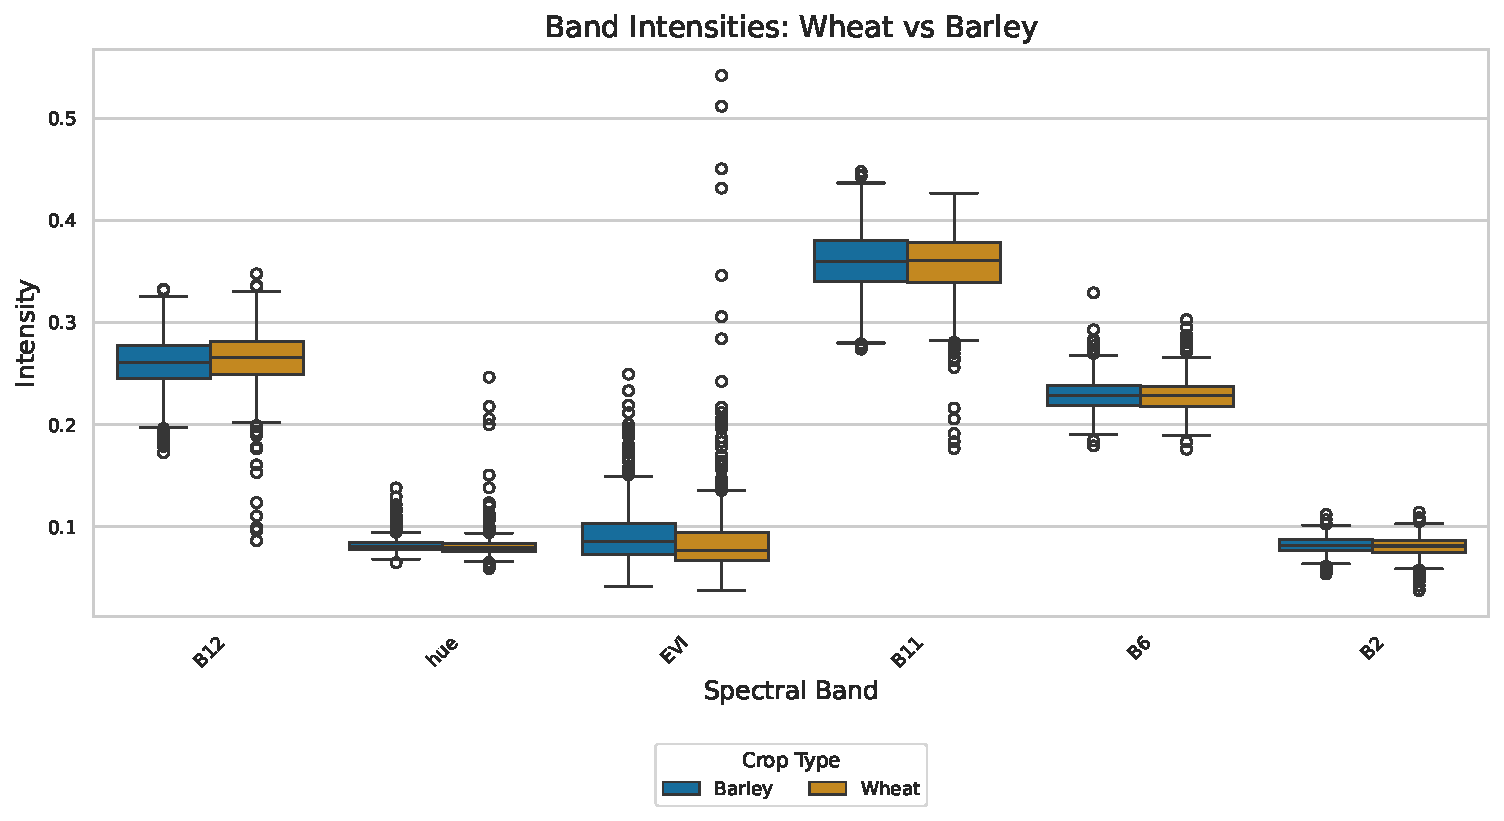
\includegraphics[width=0.55\textwidth]{wheat_barley_boxplot.pdf}
  \caption{Boxplots comparing spectral band intensities of wheat and barley, highlighting their high degree of spectral similarity and potential for classification confusion.}
  \label{fig:wheat-barley-boxplot}
\end{figure}

These findings highlight the need to incorporate temporal information that better represents phenological stages throughout the growing season to improve crop classification. The unique temporal dynamics associated with the stages of crop development (e.g., emergence, peak greenness, senescence) provide additional discriminatory power that can help resolve ambiguities between crops with similar spectral signatures \cite{wardlow2007towards}. Therefore, integrating both spectral and temporal data was crucial to enhance classification accuracy, especially in complex agricultural landscapes where crops like wheat and barley were spectrally similar.

\section{Methodology}

This study explores three complementary modeling paradigms for crop classification: feature-based machine learning, deep learning, and patch-based approaches. These paradigms differ in how spatial and temporal information from multi-spectral Sentinel-2 imagery is represented and utilized.

Classical machine learning relies on engineered features derived from pixel-level time series, while deep learning models learn hierarchical representations directly from raw data. In contrast, patch-based approaches operate on spatially contiguous regions, enabling the model to capture local spatial structure and contextual relationships that are not available in purely pixel-wise representations. Each paradigm was evaluated at both the pixel level and the field (or patch) level to assess their effectiveness across different representations of the data.

Crop classification from remote sensing data can therefore be approached through three complementary strategies: feature engineering, representation learning, and spatial context modeling.

In the feature engineering paradigm, domain knowledge is used to construct descriptive inputs from raw spectral time series. These include vegetation indices such as NDVI, spectral band ratios, textural measures, and phenological statistics, which are then used as inputs to classical machine learning models such as Random Forests (RF), Support Vector Machines (SVM), and Gradient Boosted Trees (GBT) \cite{ieee2017}. In this study, we adopt the \texttt{xr\_fresh} framework to automatically extract a comprehensive set of time-series features, enabling the construction of high-dimensional representations without manual feature design \cite{mann2025}.

In contrast, deep learning follows a representation learning paradigm, where models learn hierarchical feature representations directly from raw input data. Convolutional Neural Networks (CNNs) capture local spatial and spectral patterns, while Recurrent Neural Networks (RNNs) and Transformer-based architectures model temporal dependencies and long-range interactions in multi-temporal data \cite{acm2020}. These approaches reduce reliance on hand-crafted features and allow the model to learn complex crop growth dynamics directly from the data.

Beyond pixel-level modeling, patch-based approaches introduce an additional spatial dimension by processing contiguous regions of imagery rather than individual pixels. This enables models to capture local texture, spatial heterogeneity, and contextual relationships between neighboring pixels, which are particularly important in agricultural landscapes where crop patterns exhibit strong spatial coherence. Patch-based models therefore complement both classical and deep learning approaches by explicitly incorporating spatial context into the classification process.

This study systematically compares these paradigms to evaluate their relative strengths, computational trade-offs, and effectiveness in handling complex agricultural environments, particularly under conditions of spectral similarity and temporal variability.

Model performance was assessed using a combination of standard classification metrics, including Cohen’s Kappa, F1-score, and prediction entropy. These metrics were selected to evaluate not only overall accuracy but also class balance and prediction confidence across imbalanced crop types.

\subsection{Classical Machine Learning}
\label{sec:pixelfield}

In the classical approach, we automated feature extraction using the \texttt{xr\_fresh} toolkit to rapidly compute a comprehensive set of statistical and temporal features from each 11-month spectral time series \cite{mann2023,mann2025}. To address class imbalance, we applied SMOTE. Several classifiers such as Logistic Regression, Random Forest, LightGBM, and XGBoost were then evaluated.

\begin{figure}[ht]
  \centering
  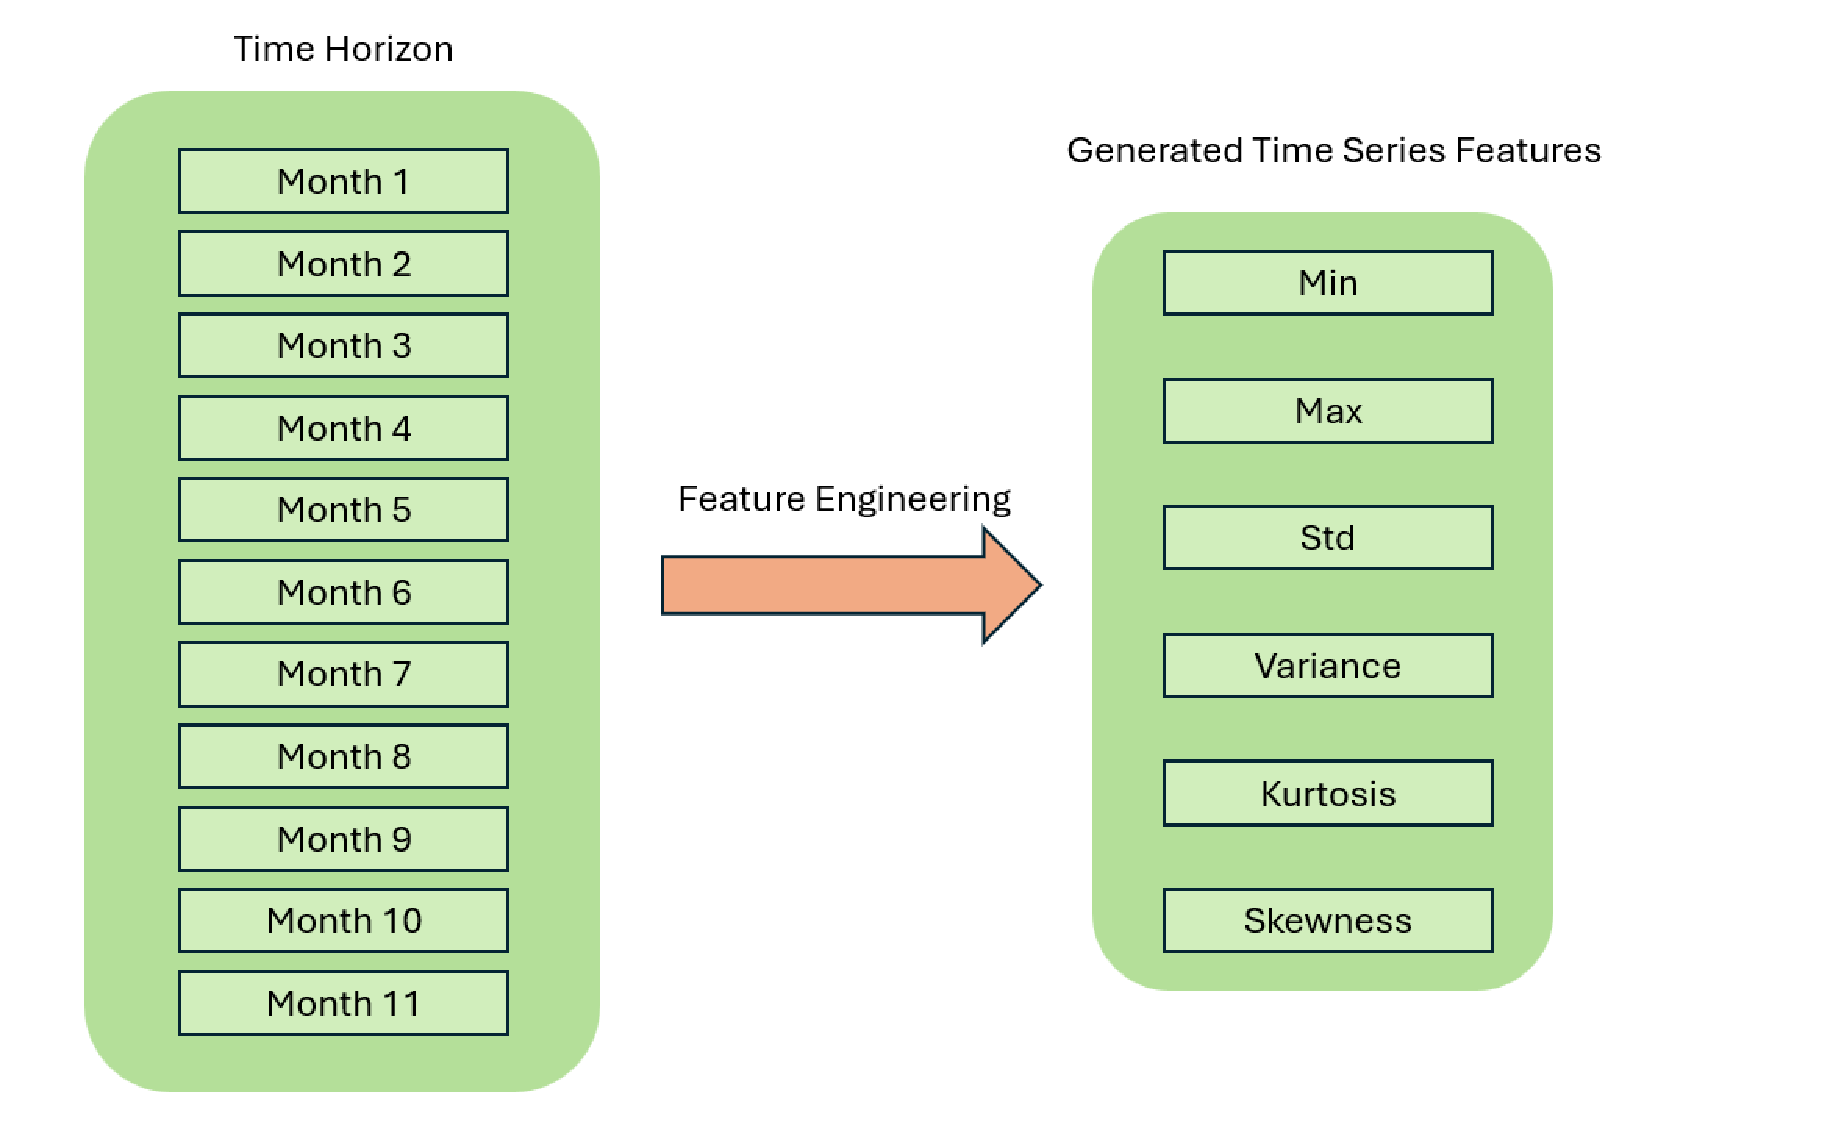
\includegraphics[width=0.55\linewidth]{Time_Series_Feature_Generation.pdf}
  \caption{Extraction of statistical and temporal features from the 11-month spectral time series.}
  \label{fig:ts_features}
\end{figure}

We extracted the following features from each pixel’s 11-month spectral profile \cite{mann2023}:
\begin{itemize}
  \item \textbf{Absolute Energy:} Sum of squared values, capturing overall signal magnitude.
  \item \textbf{Absolute Sum of Changes:} Total absolute difference between consecutive measurements, reflecting temporal variability.
  \item \textbf{Autocorrelation (1,2-month lag):} Correlation with its one- and two-month lagged versions, indicating series persistence.
  \item \textbf{Count Above Mean:} Number of points above the series mean, quantifying high-value occurrences.
  \item \textbf{Day of Year of Max/Min:} Julian day when the maximum and minimum occur, marking peak and low activity periods.
  \item \textbf{Kurtosis:} Tail heaviness of the distribution, highlighting propensity for extremes.
  \item \textbf{Linear Trend:} Slope of a least-squares fit, summarizing the overall upward or downward trend.
  \item \textbf{Longest Strike Above/Below Mean:} Longest consecutive run above or below the mean, capturing sustained periods.
  \item \textbf{Max/Min:} Absolute extreme values in the series.
  \item \textbf{Mean/Median:} Measures of central tendency.
  \item \textbf{Mean Absolute Change/Mean Change:} Average magnitude and signed change between consecutive points.
  \item \textbf{Mean Second Derivative:} Mean of the series’ second differences, detecting acceleration or deceleration.
  \item \textbf{Quantiles (0.05, 0.95):} Values at the 5th and 95th percentiles, summarizing distribution extremes.
  \item \textbf{Ratio Beyond \(r\sigma\):} Proportion of points more than \(r\) standard deviations (r=1,2,3) from the mean.
  \item \textbf{Skewness:} Asymmetry of the distribution around the mean.
  \item \textbf{Standard Deviation/Variance:} Spread measures around the mean.
  \item \textbf{Sum of Values:} Total sum of observations (mean × length).
  \item \textbf{Symmetry Looking:} Similarity when the series is reversed.
  \item \textbf{Time Series Complexity:} Complexity-Invariant Distance metric of sequence irregularity.
\end{itemize}

This toolkit allowed us to extract all required time-series features efficiently, ensuring each pixel’s temporal signature was well-represented for robust classification \cite{mann2025}.

\subsubsection{Pixel-Level Analysis}

For pixel-level analysis, each pixel was treated as an independent sample. Feature vectors from each pixel’s 11-month history were used to train classifiers. During inference, pixel predictions within a field polygon were aggregated via majority voting to determine the overall field label.

\paragraph{Baseline Classical Models:}

To benchmark crop classification, we used four classical models: Logistic Regression, Random Forest, LightGBM, and XGBoost—ranging from interpretable linear models to advanced tree-based learners.

Each pixel was represented by a feature vector $\mathbf{x}_i \in \mathbb{R}^{174}$, formed from time-series features across ten months and six spectral indices (B2, B6, B11, B12, EVI, Hue), capturing phenological signatures over time.

\paragraph{Logistic Regression (LR):}
    \[
    P(y_i = c \mid \mathbf{x}_i) =
    \frac{\exp(\mathbf{w}_c^\top \mathbf{x}_i + b_c)}
    {\sum_{c'=1}^{C} \exp(\mathbf{w}_{c'}^\top \mathbf{x}_i + b_{c'})}
    \]
  A linear model that provides interpretable weights \cite{james2013}.

\paragraph{Random Forest (RF):} 
  \[
  \hat{y}_i = \text{mode}\left\{ T_1(\mathbf{x}_i), T_2(\mathbf{x}_i), \dots, T_K(\mathbf{x}_i) \right\}
  \]
  An ensemble of decision trees that captures non-linear interactions \cite{breiman2001}.
  
\paragraph{LightGBM:}
  \[
  \hat{y}_i^{(t)} = \hat{y}_i^{(t-1)} + \eta \cdot f_t(\mathbf{x}_i)
  \]
  Gradient boosting with efficient leaf-wise learning \cite{ke2017}.

\paragraph{XGBoost:}
  \[
  \mathcal{L} = \sum_i l(y_i, \hat{y}_i) + \sum_k \Omega(f_k)
  \]
  \[
  \Omega(f_k) = \gamma T_k + \frac{1}{2}\lambda \sum_j w_j^2
  \]
  Regularized boosting to reduce overfitting \cite{chen2016, friedman2001}.

\paragraph{Pixel-Level Ensemble with Hybrid Voting:}

We ensembled RF, XGBoost, and LightGBM using soft voting. Per-pixel class probabilities were averaged:
\[
\hat{\mathbf{P}}_i = \frac{1}{3} \left( \mathbf{P}_{\text{RF}}(\mathbf{x}_i) + \mathbf{P}_{\text{XGB}}(\mathbf{x}_i) + \mathbf{P}_{\text{LGBM}}(\mathbf{x}_i) \right)
\quad
\hat{y}_i = \arg\max_k \hat{P}_i(k)
\]

\paragraph{Field-Level Aggregation:}

Let field \( f \) consist of pixels \( i \in f \). Field-level soft voting is computed as:

\[
\bar{\mathbf{P}}_f = \frac{1}{|f|} \sum_{i \in f} \hat{\mathbf{P}}_i
\quad
\hat{y}_f^{\text{soft}} = \arg\max_k \bar{P}_f(k)
\]

We introduced a confidence margin:
\[
\Delta_f = \bar{P}_f^{(1)} - \bar{P}_f^{(2)}
\]

where \(\bar{P}_f^{(1)}\) and \(\bar{P}_f^{(2)}\) are the highest and second-highest class probabilities in \(\bar{P}_f\), respectively.\\

If \( \Delta_f < \theta \) (threshold = 0.10), we fall back to mode voting across pixel labels:

\[
\hat{y}_f^{\text{mode}} = \text{mode} \left\lbrace \hat{y}_i \mid i \in f \right\rbrace
\]

\paragraph{Final Hybrid Rule:}
\[
\hat{y}_f =
\begin{cases}
\hat{y}_f^{\text{soft}}, & \text{if } \Delta_f \geq \theta \\
\hat{y}_f^{\text{mode}}, & \text{otherwise}
\end{cases}
\]

This strategy balanced probabilistic confidence with categorical consistency, improving field-level classification stability.

\subsubsection{Field-Level Analysis}
In the field-level analysis, we aggregated all pixel features within each field polygon, as shown in Figure~\ref{fig:field_aggregation}, by computing the mean across pixels to form a single representative feature vector per field. This step reduced noise and the influence of outlier pixels while preserving meaningful spatial patterns. Classifiers were then trained using these aggregated field-level vectors to directly learn from spatially coherent crop representations. This approach aligns with previous findings that object-based aggregation helps in minimizing spectral confusion and enhances classification accuracy, especially in homogeneous agricultural regions \cite{maxwell2019}.

\begin{figure}[ht]
\centering
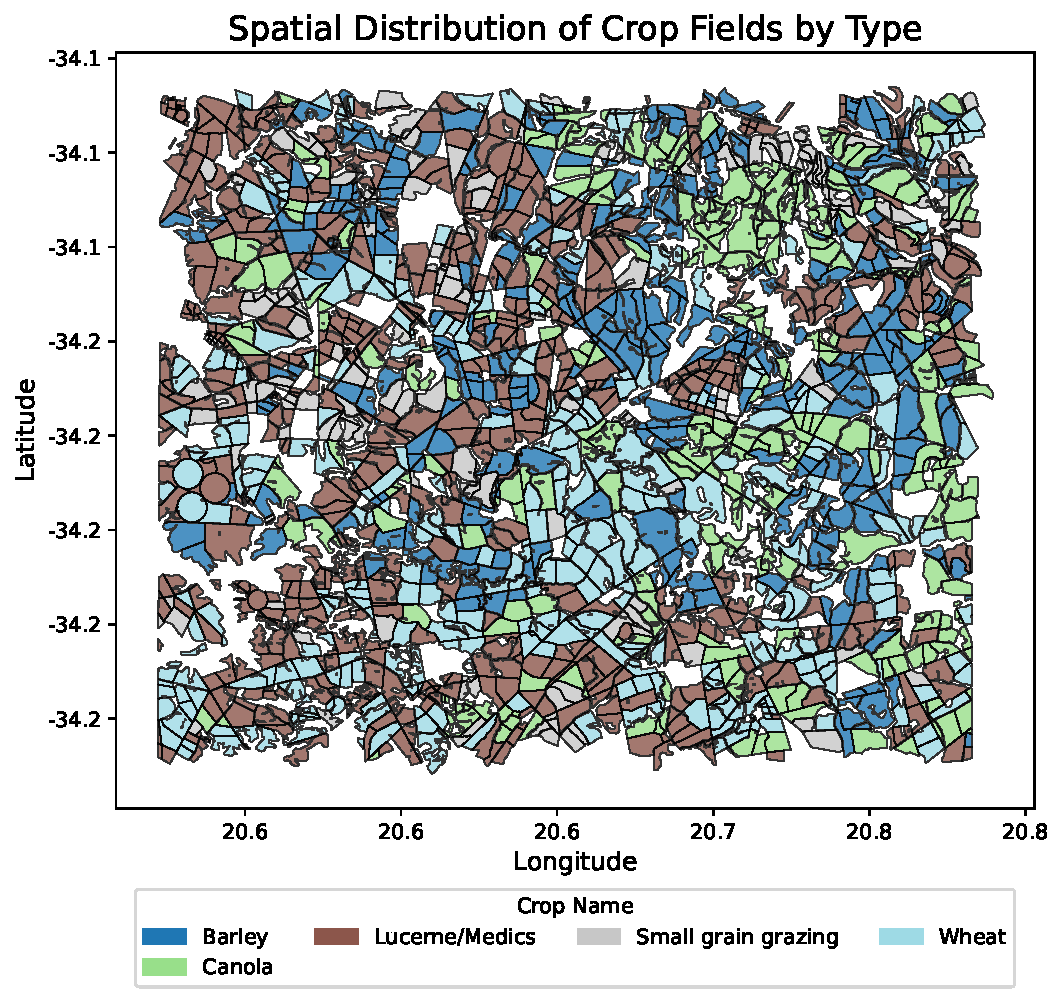
\includegraphics[width=0.55\linewidth]{field_boundaries_by_crop.pdf}
\caption{Illustration of field-level aggregation: pixel values are grouped by field polygon and summarized into a single feature vector.}
\label{fig:field_aggregation}
\end{figure}

\vspace{0.5em}

To address class imbalance at the field level, we combined \textbf{SMOTETomek} resampling with a \textbf{stacked ensemble classifier}. This approach ensured both balanced data and strong generalization performance.

\paragraph{SMOTETomek Resampling}
    SMOTETomek combines oversampling and undersampling techniques. SMOTE generates synthetic samples for underrepresented classes by interpolating between existing samples, while Tomek Links removes borderline examples to improve class separability. This helped mitigate the severe class imbalance visible in Figure~\ref{fig:EDA-1}, especially for crops like small grain grazing and canola.\\

\paragraph{Stacked Ensemble Classifier}
    We built a two-layer ensemble consisting of Random Forest and XGBoost as base learners, with Logistic Regression (using \texttt{passthrough=True}) as the meta-learner, allowing it to use both base-model predictions and the original input features. The final prediction for pixel \(i\) is defined as:
    \[
    \hat{y}_i^{\text{stacked}} = f_{\text{meta}}\left(f_{\text{RF}}(\mathbf{x}_i),\; 
    f_{\text{XGB}}(\mathbf{x}_i),\; \mathbf{x}_i\right)
    \]
    This architecture combines the non-linear modeling capacity of tree-based learners with a linear meta-learner that integrates both base predictions and original input features.\\

\paragraph{Field-Based Aggregation and XGBoost Optimization}
    We also implemented an optimized field-level pipeline using XGBoost. Field identifiers were used to ensure that no field contributed to more than one data split, with fields split into train/validation/test sets using \texttt{fid}-based stratification. Features were aggregated via the mean across pixels, and labels via the mode crop type per field.

    Optuna was then used to tune XGBoost over 75 trials, searching across  \texttt{n\_estimators}, \texttt{max\_depth}, \texttt{learning\_rate}, \texttt{subsample}, \texttt{colsample\_bytree}, \texttt{gamma}, \texttt{reg\_alpha}, \texttt{reg\_lambda}, and \texttt{min\_child\_weight}, with the objective of maximizing the weighted F1 score via 5-fold stratified cross-validation. The best configuration (Trial 32) is detailed in Table~\ref{tab:top5_trials}, which also achieved a validation accuracy of 76.61\%.

\begin{table}[htbp]
\centering
\scriptsize % Further reduce font size
\caption{Top 5 trials from hyperparameter search with corresponding parameters and validation accuracies}
\label{tab:top5_trials}
\renewcommand{\arraystretch}{1.1}
\setlength{\tabcolsep}{3pt} % Tight column spacing
\begin{tabular}{ccccccccccc}
\toprule
\textbf{Trial} & \textbf{Acc.} & \textbf{Est.} & \textbf{Depth} & \textbf{LR} & \textbf{SubS} & \textbf{ByTree} & \textbf{Gamma} & \textbf{Reg$\alpha$} & \textbf{Reg$\lambda$} & \textbf{MinCW} \\
\midrule
32 & \textbf{76.61\%} & 1141 & 13 & 0.0215 & 0.5749 & 0.6986 & 0.5589 & 0.00184 & 0.00259 & 5 \\
12 & 76.46\% & 984  & 12 & 0.0145 & 0.6675 & 0.6946 & 0.0799 & 0.00503 & 0.00455 & 7 \\
24 & 76.40\% & 1165 & 11 & 0.0162 & 0.7831 & 0.6403 & 0.00413 & 0.00481 & 0.00478 & 9 \\
13 & 76.29\% & 995  & 12 & 0.0277 & 0.6345 & 0.6829 & 0.3999 & 0.00011 & 0.00567 & 6 \\
18 & 76.29\% & 915  & 13 & 0.0121 & 0.6784 & 0.5958 & 0.1612 & 0.00491 & 0.1732 & 8 \\
\bottomrule
\end{tabular}
\end{table}

\subsection{Deep Learning Architectures for Crop Classification}

Deep learning models ingest raw spectral values and learn hierarchical representations
that capture both spatial and temporal dependencies, offering an alternative to the
manual feature engineering required by classical approaches~\cite{maxwell2019,zhu2017,li2019}.
We explore architectures across two spatial granularities: pixel-level models that
operate on per-pixel temporal sequences, and patch-level models that additionally
exploit local spatial structure. To ensure unbiased evaluation across all architectures,
all pixels belonging to a given field were assigned exclusively to either the training,
validation, or test set, preventing spatial information leakage between splits.

% ---------------------------------------------------------------
\subsubsection{Pixel-Level Architectures}
% ---------------------------------------------------------------

At the pixel level, each sample is an individual pixel characterized by 60 temporal
features spanning the 2017 growing season — six spectral bands and vegetation
indices (B2, B6, B11, B12, EVI, Hue) observed across 10 monthly composites.
Each pixel is linked to a unique field identifier and labeled according to the
field crop type across five classes: wheat, barley, canola, small grain grazing,
and lucerne/medics. Pixel-level predictions are subsequently aggregated to the
field level via majority voting:
\[
    \hat{y}_{f} = \operatorname{mode}\!\left(\{\hat{y}_{i} \mid i \in f\}\right)
\]
For TabNet models we applied z-score standardization; CNN-based models were
trained on raw reflectance values, allowing convolutional layers to learn directly
from temporal magnitude patterns.

% --- 1. CNN + BiLSTM ---
\paragraph{CNN + BiLSTM Ensemble with Focal Loss.}

To capture the intricate temporal dynamics of crop growth, we developed a hybrid
architecture combining 1D Convolutional Neural Networks (CNNs) with Bidirectional
Long Short-Term Memory (BiLSTM) networks (Figure~\ref{fig:cnn_bilstm}).

\begin{figure}[htbp]
\centering
\includegraphics[width=0.55\textwidth]{cnn_bilstm.pdf}
\caption{Architecture of the CNN + BiLSTM model. The model combines 1D
convolutional temporal feature extraction with sequential modeling through a
BiLSTM layer.}
\label{fig:cnn_bilstm}
\end{figure}

The model processes an input tensor of shape $(B, 6, T)$. A 1D convolutional
layer with 64 filters and kernel size 5 is applied along the temporal axis,
followed by ReLU activation and tensor permutation to $(B, T, 64)$ for
compatibility with the recurrent layer. A bidirectional LSTM with hidden size
64 then captures temporal dependencies in both forward and backward directions,
yielding an output of shape $(B, T, 128)$. The representation at the final
timestep passes through dropout and a fully connected layer, with class
probabilities computed via softmax:
\[
    P(y_i = c \mid \mathbf{x}_i)
    = \frac{e^{z_{i,c}}}{\sum_{c'=1}^{C} e^{z_{i,c'}}}
\]

To address class imbalance we used Focal Loss:
\[
    \mathcal{L}_{\text{focal}} = -\alpha_t (1 - p_t)^{\gamma} \log(p_t)
\]
where $\alpha_t$ is the class weighting factor and $\gamma = 2.0$ is the focusing
parameter. A \texttt{WeightedRandomSampler} further
ensured balanced class representation during training. To reduce variance, five
identical models were trained with different random seeds and their logits averaged:
\[
    \text{Logits}_{\text{ensemble}}
    = \frac{1}{N} \sum_{k=1}^{N} \text{Logits}^{(k)}
\]

% --- 2. TabNet ---
\paragraph{Ensemble of TabNet Models.}

TabNet treats satellite observations as structured tabular inputs — each pixel's
repeated measurements organized as a flat feature vector — and learns through
iterative attention-based feature selection rather than temporal ordering
(Figure~\ref{fig:tabnet_architecture}). At each decision step, an Attentive
Transformer generates a sparse mask selecting the most relevant input dimensions,
which are then transformed by a Feature Transformer. This enables the model to
focus on different feature subsets at different depths without relying on
explicit temporal structure~\cite{tabnet2024}.

\begin{figure}[htbp]
\centering
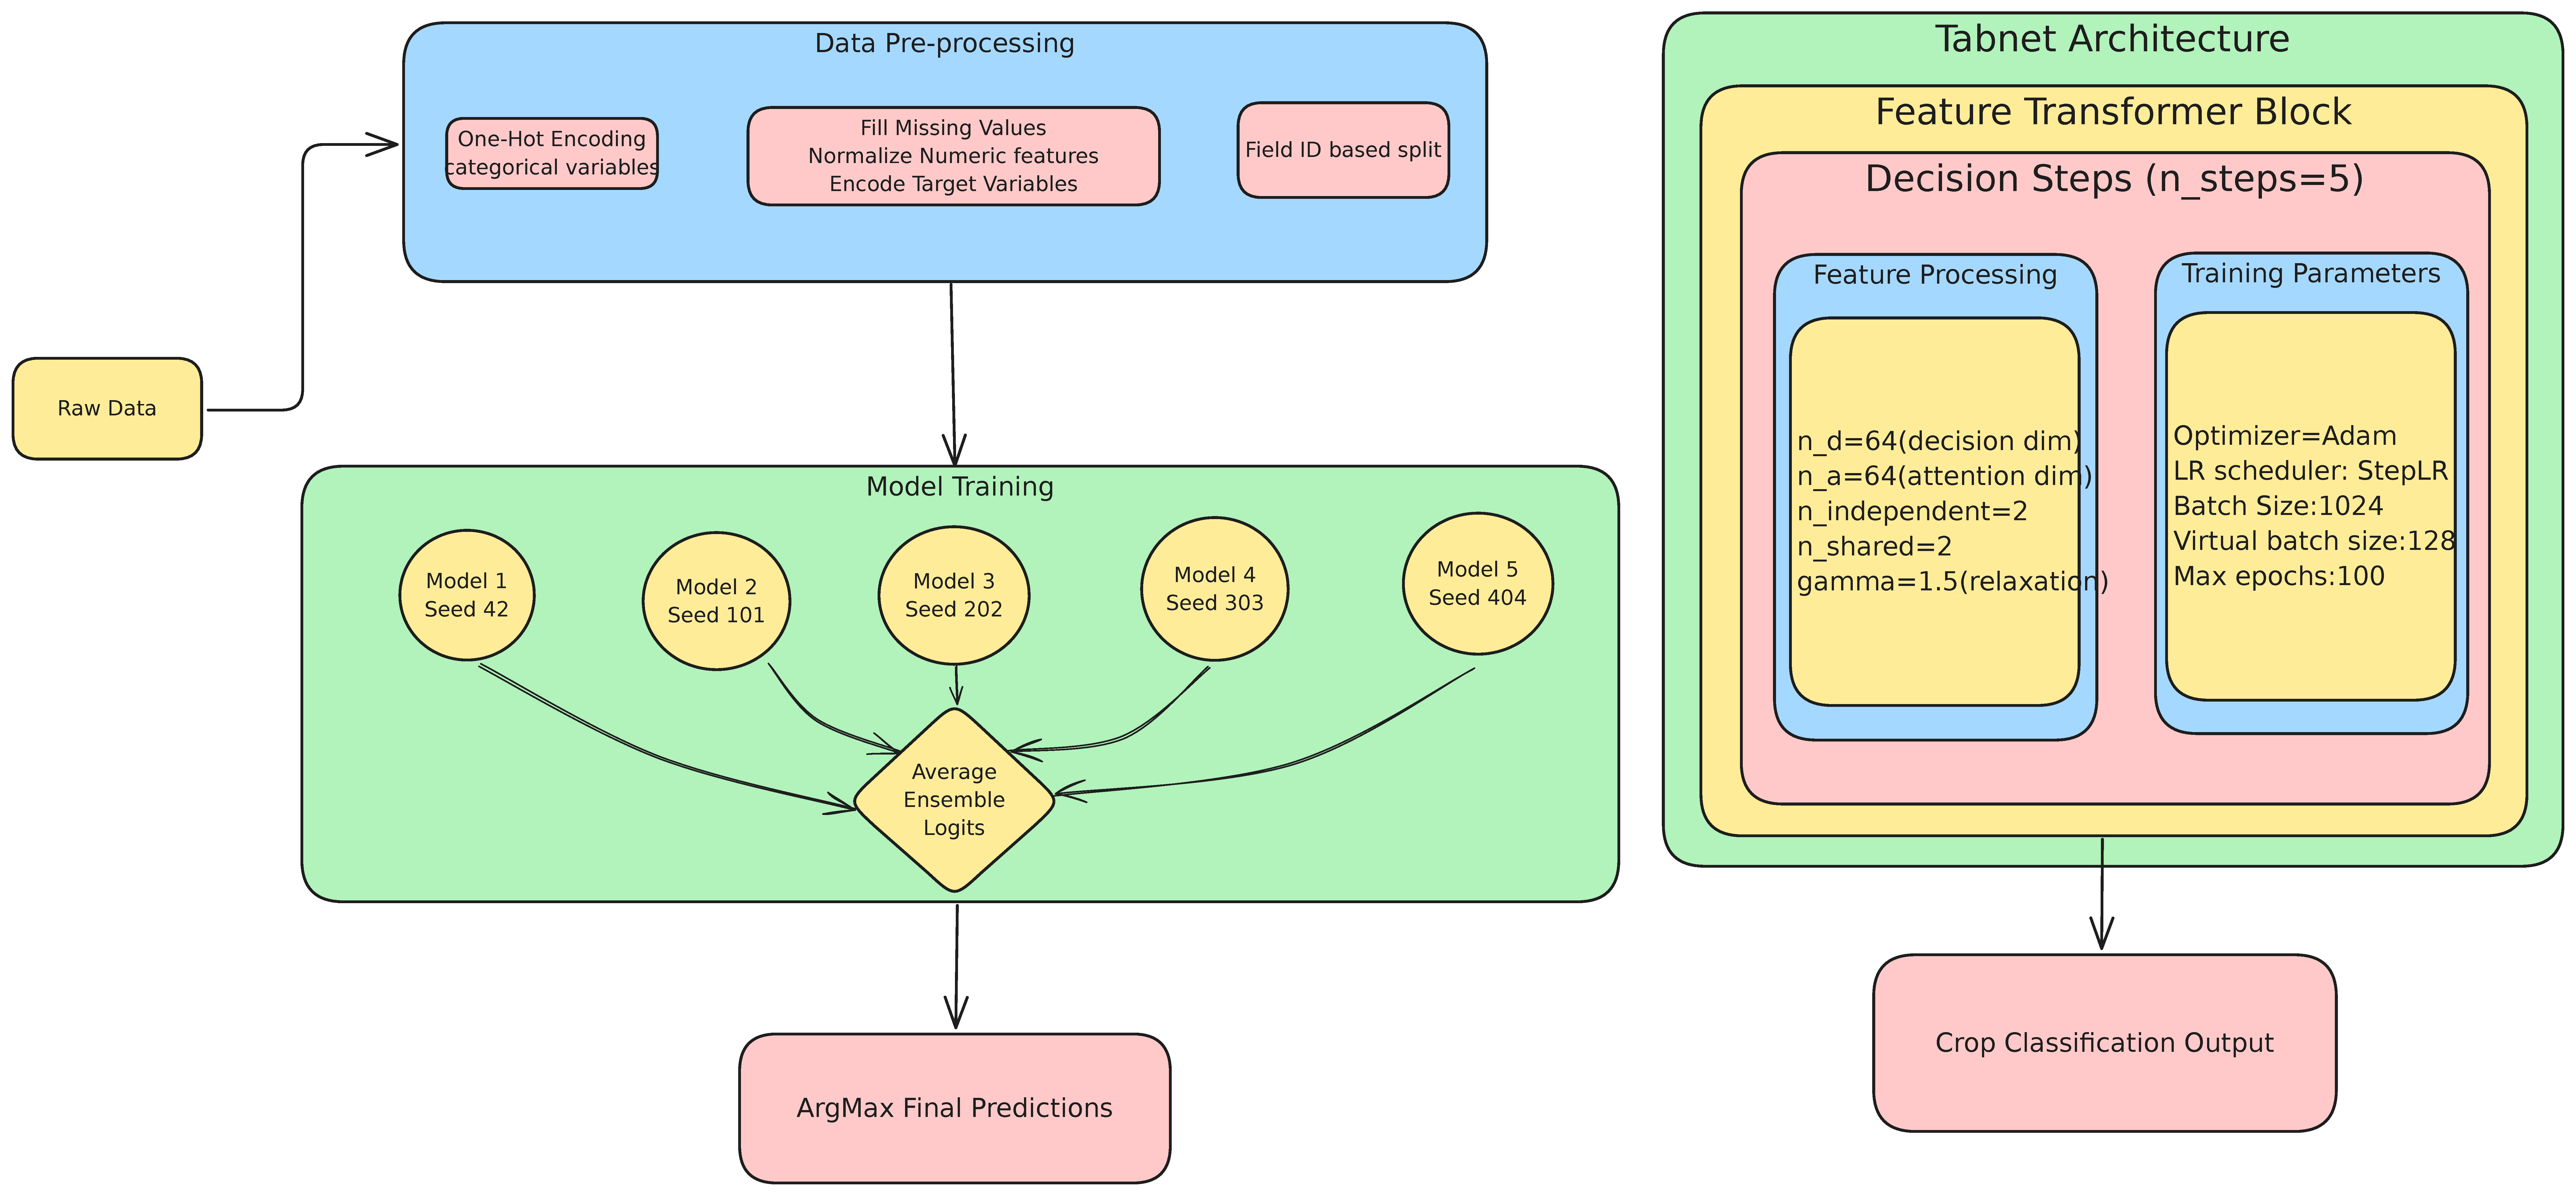
\includegraphics[width=0.55\textwidth]{tabnet.pdf}
\caption{Architecture of the TabNet ensemble. Each model applies iterative
attention-based feature selection. Final predictions are obtained by averaging
softmax outputs across five models, followed by field-level majority voting.}
\label{fig:tabnet_architecture}
\end{figure}

The network used $n_d = n_a = 64$, independent and shared block widths of 2,
relaxation parameter $\gamma = 1.5$, and 5 decision steps. Training used the
Adam optimizer with a StepLR scheduler, batch size 1024, virtual batch size
128, and early stopping monitored on a field ID-stratified validation set.

An ensemble of five TabNet models, each initialized with a distinct random seed
(42, 101, 202, 303, 404), averaged softmax outputs to yield final class
probabilities:
\[
    \hat{\mathbf{p}}_{\text{ensemble}}
    = \frac{1}{5}\sum_{i=1}^{5}\operatorname{Softmax}\!\left(\mathbf{z}^{(i)}\right),
    \qquad
    \hat{y} = \arg\max_c\,\hat{p}_{\text{ensemble},c}
\]
A practical advantage of TabNet is interpretability: the sparse decision masks
can be inspected post hoc to identify which spectral bands or vegetation indices
most influenced each prediction~\cite{tabnet2024}.

% --- 3. 1D CNN ---
\paragraph{1D CNN with Optuna Hyperparameter Tuning.}

As a lightweight baseline we implemented a 1D CNN whose architecture was
optimized via Optuna~\cite{cnn_optuna} (Figure~\ref{fig:cnn_architecture}).
The input is reshaped to $(B, 6, T)$, representing six spectral channels across
monthly intervals, and passed through a single convolutional layer followed by
ReLU, adaptive average pooling, dropout, and a fully connected classification
head. The hyperparameter optimization objective was:
\[
    \theta^* = \arg\max_{\theta \in \mathcal{H}}\,\mathcal{A}_{\text{val}}(f_\theta)
\]
where $\theta = \{\text{lr},\,\text{dropout},\,\text{filters},\,\text{kernel size}\}$,
solved using the Tree-structured Parzen Estimator (TPE). Each trial was evaluated
over 25 epochs with a class-weighted sampler. The best configuration (Table~\ref{tab:optuna_top_trials})
used a kernel size of 7, 64 filters, dropout $\approx 0.49$, and learning rate
0.00116, yielding a validation accuracy of 75.5\%.

\begin{figure}[htbp]
\centering
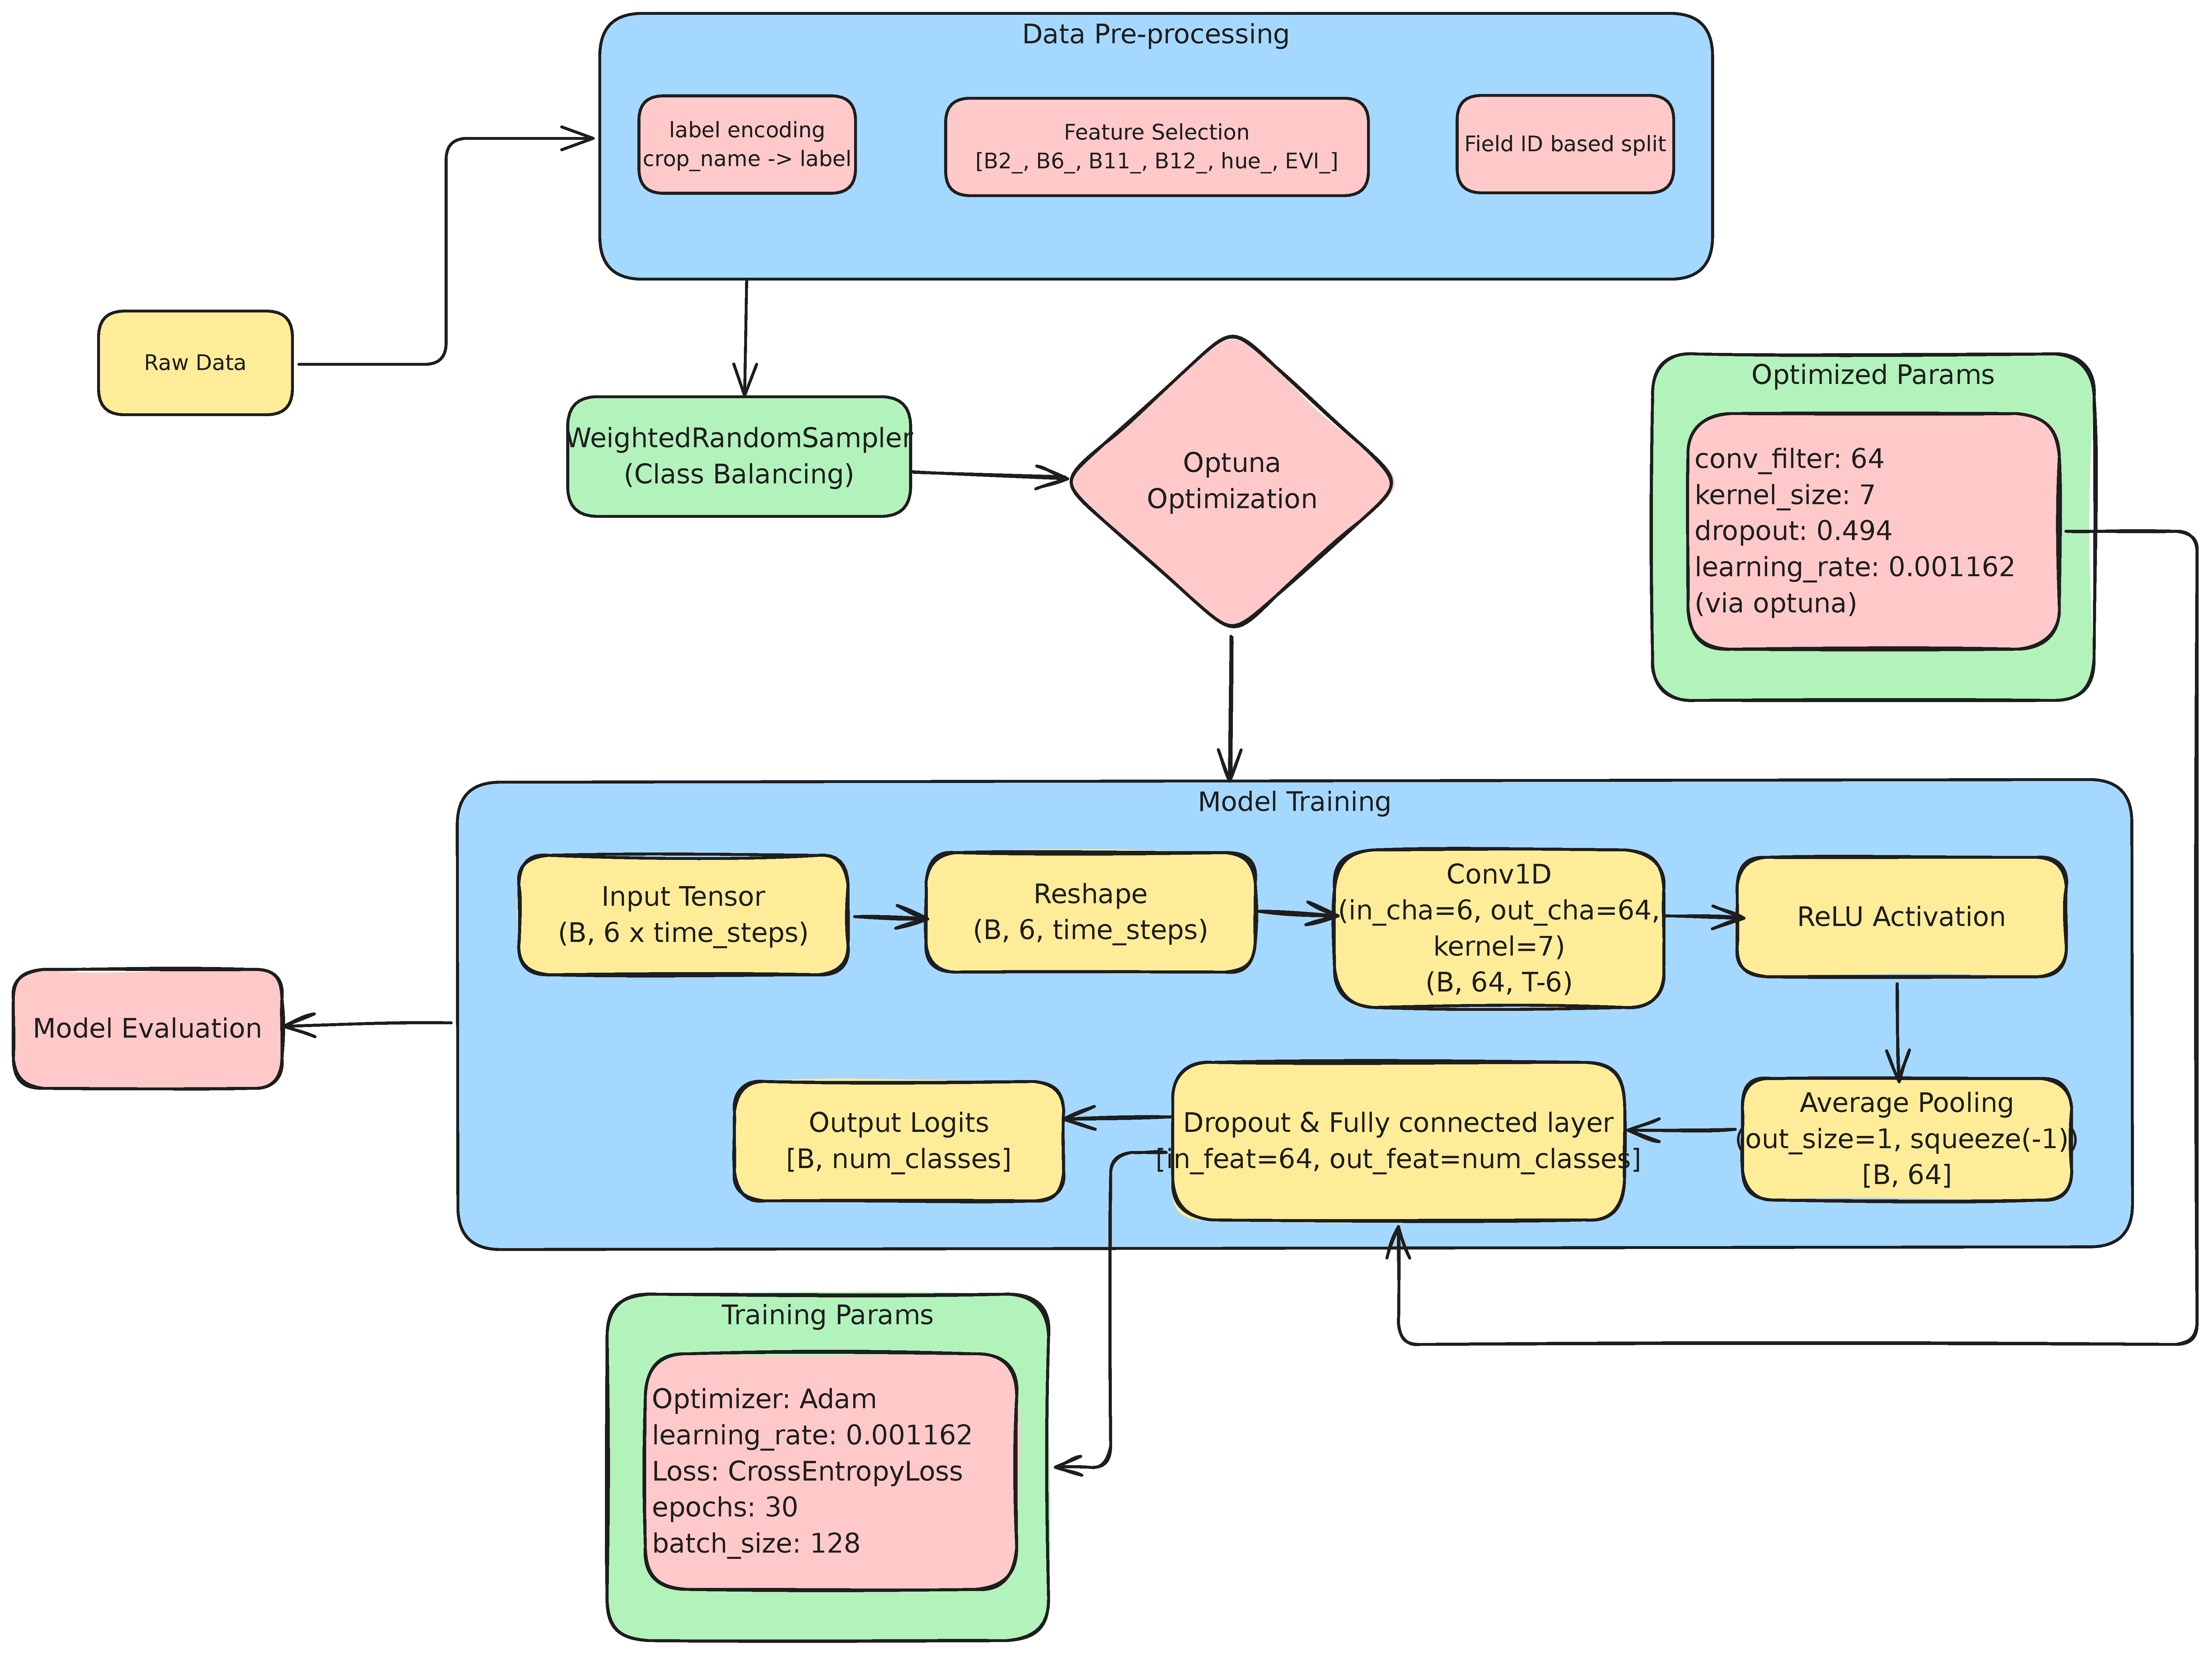
\includegraphics[width=0.55\textwidth]{cnn_hyper.pdf}
\caption{Architecture of the 1D CNN model optimized via Optuna: a single
convolutional layer followed by ReLU activation, adaptive pooling, and a
fully connected classification head.}
\label{fig:cnn_architecture}
\end{figure}

\begin{table}[htbp]
\centering
\caption{Top Optuna trials for the 1D CNN ranked by validation accuracy.}
\label{tab:optuna_top_trials}
\renewcommand{\arraystretch}{1.1}
\setlength{\tabcolsep}{4pt}
\begin{tabular}{cccccc}
\toprule
\textbf{Trial} & \textbf{Val.\ Acc.} & \textbf{LR} & \textbf{Dropout}
    & \textbf{Filters} & \textbf{Kernel} \\
\midrule
14 & \textbf{75.53\%} & 0.00116 & 0.5 & 64  & 7 \\
13 & 74.06\%           & 0.00102 & 0.5 & 128 & 7 \\
19 & 74.61\%           & 0.00118 & 0.4 & 64  & 7 \\
7  & 73.20\%           & 0.00013 & 0.3 & 128 & 7 \\
11 & 73.66\%           & 0.00006 & 0.4 & 128 & 7 \\
\bottomrule
\end{tabular}
\end{table}

% ---------------------------------------------------------------
\subsubsection{Patch-Level Architectures}
% ---------------------------------------------------------------

To exploit local spatial structure, we transitioned to a patch-level analysis in
which each field is divided into a grid of fixed-size square patches, each
retaining the full 10-month spectral history for every pixel
(Figure~\ref{fig:example_patches}). Compared with pixel-level models, this
approach encodes spatial relationships between neighbouring pixels and provides
implicit data augmentation by generating multiple training samples per field.
The trade-off is increased computational cost and the omission of boundary
pixels that fall outside the patch grid.

\begin{figure}[H]
\centering
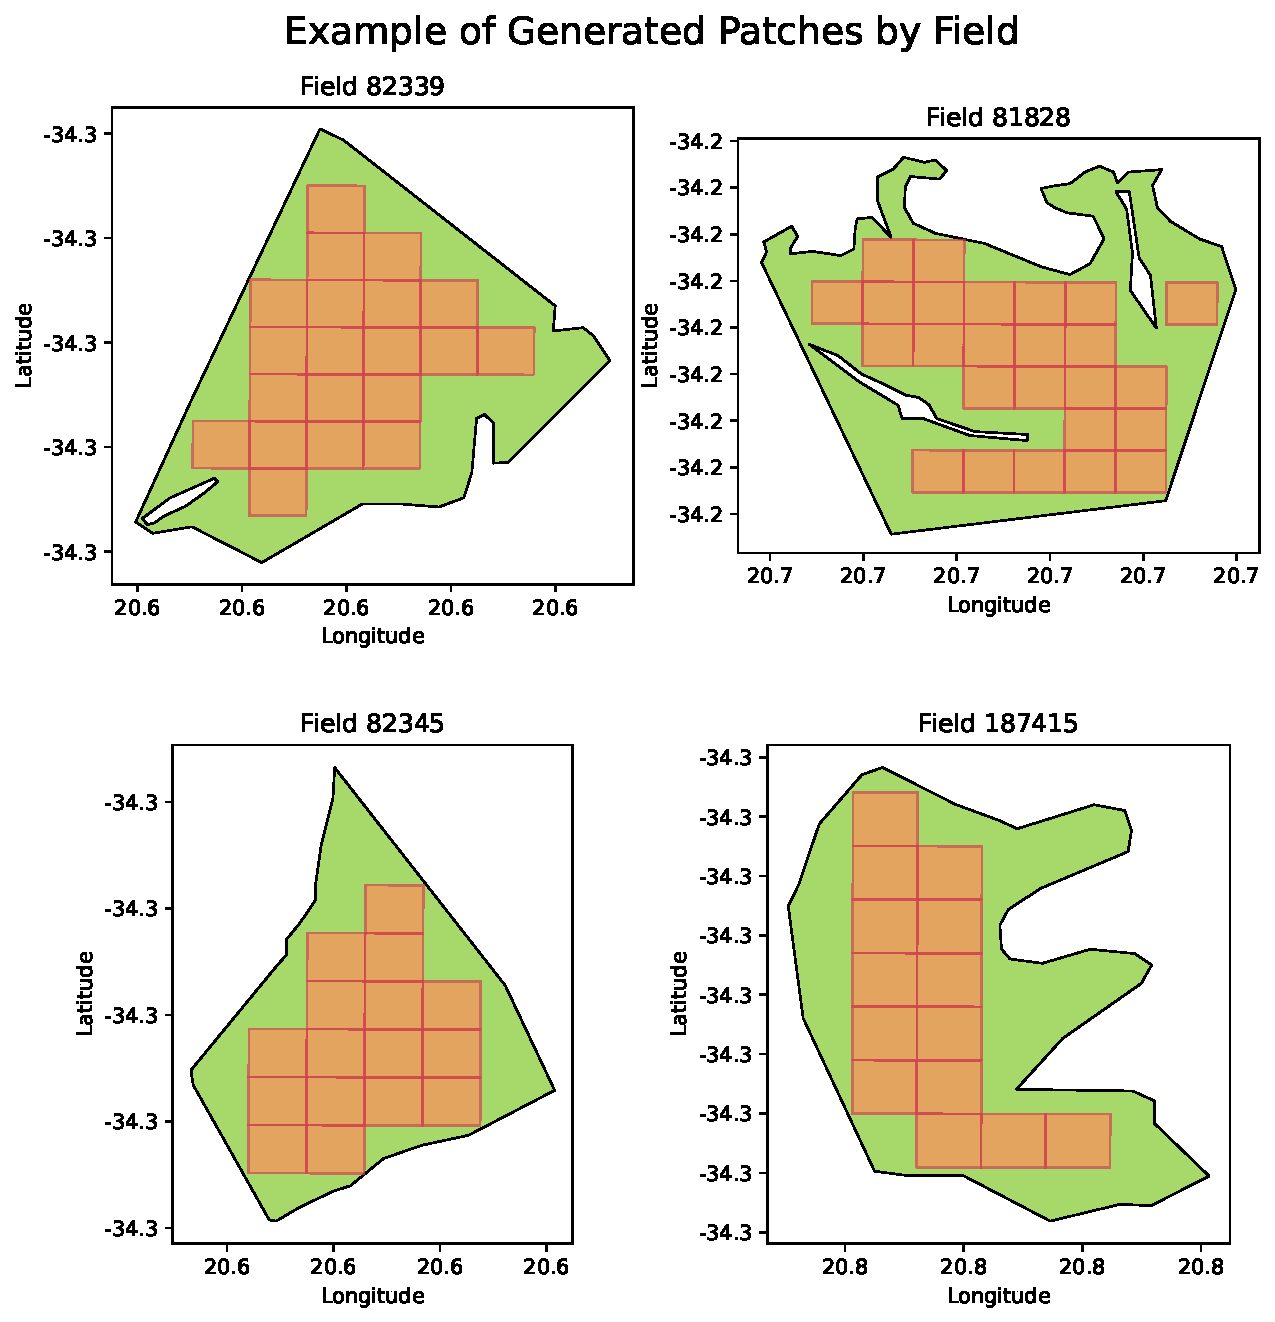
\includegraphics[width=0.55\linewidth]{Example_patches.pdf}
\caption{Illustration of patch generation per field.}
\label{fig:example_patches}
\end{figure}

We investigated three distinct patch-based architectures.

% --- 3a. Multi-Channel 2D CNN ---
\paragraph{Multi-Channel 2D CNN.}

Each spectral band and monthly observation is treated as a separate input channel,
giving a patch tensor $\mathbf{X} \in \mathbb{R}^{H \times W \times C}$
($H = W = 128$, $C = 66$). Two Conv2D blocks with $K$ filters each compute:
\[
    Y_k[i,j] = \operatorname{ReLU}\!\left(
        \sum_{c=1}^{C}\sum_{m=-1}^{1}\sum_{n=-1}^{1}
        W_{k,c,m,n}\cdot X[i+m,\,j+n,\,c] + b_k
    \right)
\]
The feature map is flattened to $\mathbf{z} \in \mathbb{R}^{128}$ and passed to
a fully connected classification head:
\[
    \hat{\mathbf{p}} = \operatorname{softmax}\!\left(W_{\mathrm{fc}}\,\mathbf{z} + b_{\mathrm{fc}}\right)
\]

% --- 3b. Ensemble of Class-Specific 3D CNNs ---
\paragraph{Ensemble of Class-Specific 3D CNNs.}

Five class-specific 3D CNNs are trained, each producing a scalar score
$p_i = f_i(\mathbf{X})$ for its target class. A logistic regression meta-learner
combines these scores into a final prediction (Figure~\ref{fig:patch_model}):
\[
    \hat{\mathbf{p}} = \operatorname{softmax}\!\left(
        W_{\mathrm{meta}}[p_1,\dots,p_5]^\top + b_{\mathrm{meta}}
    \right)
\]
By modelling volumetric relationships jointly across spectral bands, spatial
dimensions, and time, 3D convolutions capture crop-specific texture and
phenological trajectories that 2D methods treat independently.

\begin{figure}[ht]
\centering
\includegraphics[width=0.55\linewidth]{patch_model.pdf}
\caption{3D CNN ensemble architecture for patch-level crop classification.}
\label{fig:patch_model}
\end{figure}

% --- 3c. Transformer ---
\paragraph{Transformer-Based Model.}

Each patch is represented as a sequence of multi-temporal image tensors
of shape $(T, H, W, B)$, where $T$ is the number of temporal observations,
$H \times W$ is the spatial resolution (128 $\times$ 128), and $B$ is the number
of spectral bands and indices.

For each time step, a lightweight convolutional encoder is applied using a
$1 \times 1$ convolution followed by global average pooling to produce a compact
feature vector $\mathbf{z}_t \in \mathbb{R}^{d}$, where $d = 32$ in our implementation.
This results in a temporal sequence of patch-level embeddings
$\{\mathbf{z}_t\}_{t=1}^{T}$.

To incorporate temporal order, learned positional embeddings are added:
\[
\tilde{\mathbf{z}}_t = \mathbf{z}_t + \mathbf{e}_t
\]

The resulting sequence is processed using stacked Transformer encoder blocks,
each consisting of multi-head self-attention, residual connections, dropout,
and a position-wise feedforward network:
\[
\operatorname{Attention}(Q, K, V)
= \operatorname{softmax}\!\left(\frac{QK^\top}{\sqrt{d_k}}\right)V
\]

where $Q = \mathbf{Z}W_Q$, $K = \mathbf{Z}W_K$, and $V = \mathbf{Z}W_V$.

Finally, the encoded sequence is aggregated via global average pooling across
time and passed through a fully connected layer with softmax activation to
produce class probabilities:
\[
\hat{\mathbf{p}} = \operatorname{softmax}(W \cdot \mathbf{h} + b)
\]

This architecture emphasizes temporal dependency modeling across monthly
patch representations, while spatial information is incorporated indirectly
through the convolutional preprocessing stage.

\subsection{Performance Metrics}
\label{subsec:performance_metrics}

To account for the highly imbalanced class distribution in our data, we report three metrics that are more informative than overall accuracy:

\textbf{Cohen’s Kappa (Kappa)}  
    Measures agreement between predicted and true labels, corrected for chance:
    \[
    \kappa = \frac{p_o - p_e}{1 - p_e}
    \]
    where
    \[
    p_o = \frac{\text{number of correct predictions}}{N}, \quad
    p_e = \sum_{c=1}^C \left( \frac{n_{c,\text{true}}}{N} \times \frac{n_{c,\text{pred}}}{N} \right)
    \]

\textbf{Weighted F1 Score (F1)}  
    The harmonic mean of precision and recall, weighted by the support of each class:
    \[
    \mathrm{F1}_{\mathrm{weighted}} = \sum_{c=1}^C \frac{n_c}{N}
        \cdot
        \frac{2 \cdot \text{Precision}_c \cdot \text{Recall}_c}{\text{Precision}_c + \text{Recall}_c}
    \]
    where \(n_c\) is the number of true instances of class \(c\).

\textbf{Log Loss (Cross-Entropy)}  
    Quantifies the average surprise of the predicted probabilities:
    \[
    \mathrm{LogLoss} = -\frac{1}{N}\sum_{i=1}^N \sum_{c=1}^{C}
         y_{i,c}\,\ln\bigl(p_{i,c}\bigr)
    \]
    where \(y_{i,c}\in\{0,1\}\) is the one-hot true label for sample \(i\) in class \(c\), and \(p_{i,c}\) is the model’s predicted probability for that class.


We avoid reporting plain accuracy here because an imbalanced test set can yield deceptively high accuracy simply by predicting the majority class. In contrast, Cohen’s Kappa and the weighted F1 score reward correct classification across all classes. Higher values indicate better agreement and balanced precision/recall, while log loss measures prediction uncertainty—lower values indicate more confident, accurate probability estimates.

\section{Results}

All models were evaluated on an independent held-out test set. Because the class
distribution is heavily imbalanced, we report Cohen's Kappa, weighted F1, and
log-loss (entropy) rather than overall accuracy, as these metrics reward correct
classification across all classes rather than rewarding prediction of the majority
class.

% ================================================================
\subsection{Classical Machine Learning}
% ================================================================

\subsubsection{Pixel-Level Results}

Table~\ref{tab:cl_ml_pixel_results} summarizes pixel-level performance for the
classical models. Random Forest achieves the highest performance at this level,
with a Cohen's Kappa of 0.69 and an F1 score of 0.77. The boosting methods
(XGBoost and LightGBM) are competitive but fall slightly short, while Logistic
Regression and the pixel-level Voting Classifier trail the individual tree
ensembles — suggesting that soft voting over pixel probabilities before
field-level aggregation is less effective than aggregating stronger individual
models. Figure~\ref{fig:conf_rf_pixel} shows the corresponding confusion matrix.
Lucerne/medics is classified well (95.7\%), whereas small grain grazing is the
most problematic class, with over 37\% of fields misclassified as lucerne/medics
and only 36.4\% correctly identified — a pattern that persists across all models
and reflects the spectral-temporal similarity between these classes.

\begin{table}[htbp]
\centering
\caption{Out-of-sample performance for classical ML models at the pixel level.
\dag\ denotes the best-performing model at this level.}
\label{tab:cl_ml_pixel_results}
\renewcommand{\arraystretch}{1.1}
\setlength{\tabcolsep}{6pt}
\begin{tabular}{lccc}
\toprule
\textbf{Model} & \textbf{Kappa} & \textbf{F1} & \textbf{Entropy} \\
\midrule
XGBoost             & 0.68 & 0.76 & 8.47 \\
LightGBM            & 0.66 & 0.74 & 8.90 \\
Random Forest\textsuperscript{\dag} & 0.69 & 0.77 & 7.99 \\
Logistic Regression & 0.65 & 0.73 & 9.07 \\
Voting Classifier   & 0.63 & 0.72 & 9.47 \\
\bottomrule
\end{tabular}
\end{table}

\begin{figure}[htbp]
\centering
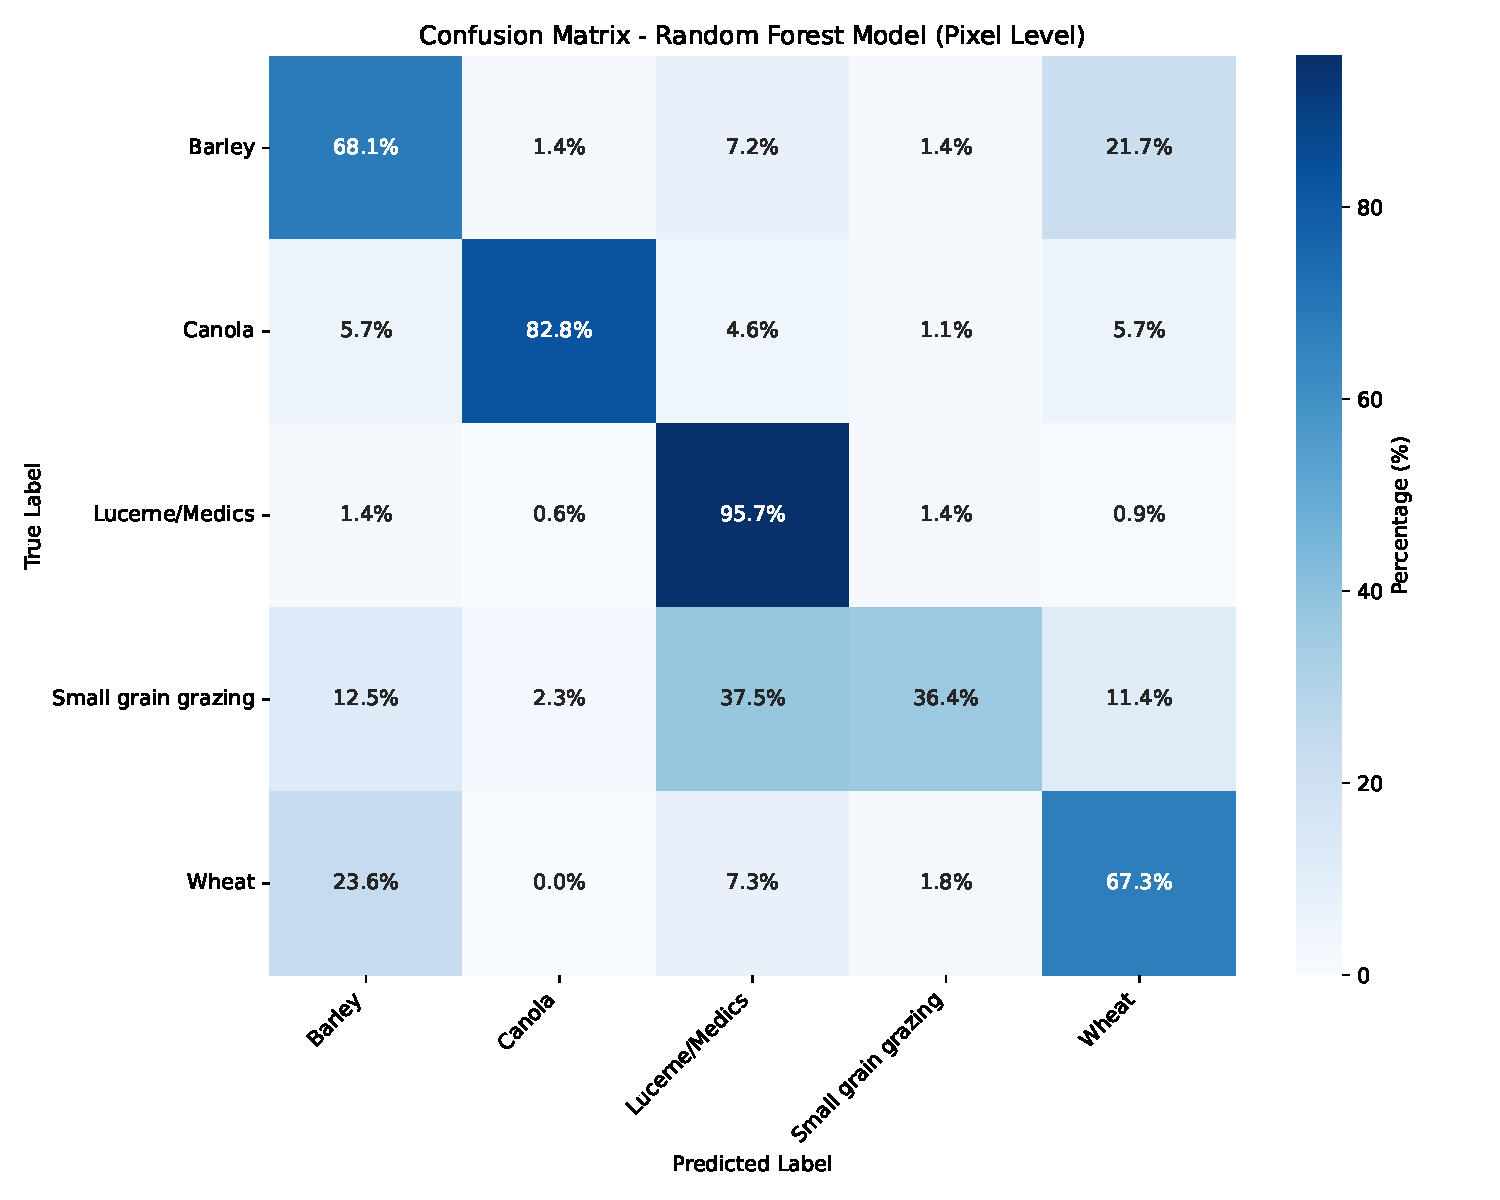
\includegraphics[width=0.55\linewidth]{confusion_matrix_rf_pixel.pdf}
\caption{Confusion matrix for Random Forest at the pixel level.}
\label{fig:conf_rf_pixel}
\end{figure}

\subsubsection{Field-Level Results}

Table~\ref{tab:ml_field_results} presents field-level performance after
aggregating pixel predictions via the hybrid soft/mode voting rule. The Voting Classifier achieves the best result
(Kappa 0.69, F1 0.76), narrowly ahead of Random Forest and LightGBM (both 0.67
Kappa). The improvement of the Voting Classifier relative to its pixel-level
performance (0.63 Kappa) illustrates the benefit of field-level aggregation for
ensemble methods: averaging probabilities across many pixels within a field
smooths out per-pixel noise and corrects individual misclassifications.

\begin{table}[htbp]
\centering
\caption{Out-of-sample performance for classical ML models at the field level.
\dag\ denotes the best-performing model at this level.}
\label{tab:ml_field_results}
\renewcommand{\arraystretch}{1.1}
\setlength{\tabcolsep}{6pt}
\begin{tabular}{lccc}
\toprule
\textbf{Model} & \textbf{Kappa} & \textbf{F1} & \textbf{Entropy} \\
\midrule
XGBoost             & 0.65 & 0.74 & 8.95 \\
LightGBM            & 0.67 & 0.76 & 8.29 \\
Random Forest       & 0.67 & 0.76 & 8.25 \\
Logistic Regression & 0.64 & 0.74 & 9.03 \\
Voting Classifier\textsuperscript{\dag} & 0.69 & 0.76 & 7.86 \\
Stacking Classifier & 0.67 & 0.75 & 8.55 \\
\bottomrule
\end{tabular}
\end{table}

Figures~\ref{fig:conf_field_stacking} and~\ref{fig:conf_field_voting} show the
field-level confusion matrices for the Stacking and Voting ensembles. Both
exhibit strong diagonal dominance. For the Stacking Ensemble, lucerne/medics
reaches 94.6\% accuracy, but small grain grazing remains poorly classified at
31.1\%, with substantial confusion into lucerne/medics (28.4\%) and wheat
(25.7\%). The Voting Ensemble improves lucerne/medics to 97.2\% and reduces
misclassification rates for barley and small grain grazing, suggesting that
consensus-based aggregation is more robust than the stacking meta-learner for
this dataset. Wheat classification improves from 55.6\% to 57.0\%, though
confusion with barley persists across both ensembles, consistent with the
spectral similarity documented in Figure~\ref{fig:wheat-barley-boxplot}.

\begin{figure}[htbp]
\centering
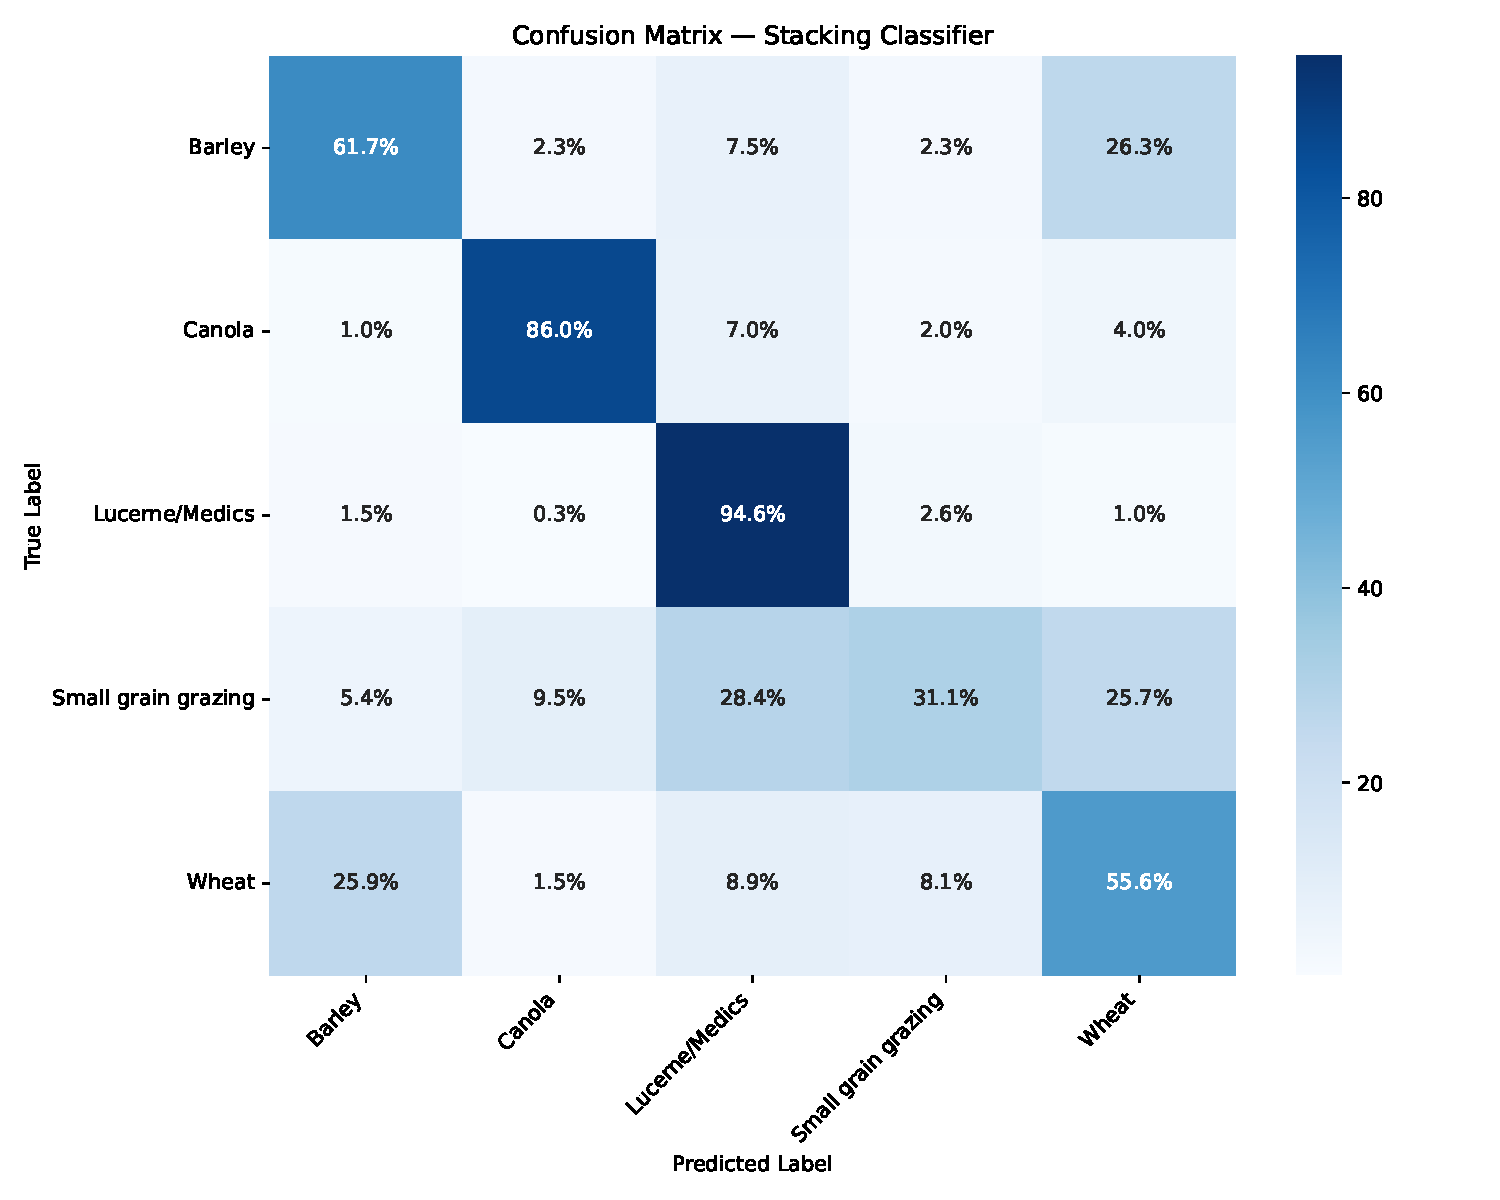
\includegraphics[width=0.55\linewidth]{confusion_matrix_Stacking_Classifier.pdf}
\caption{Confusion matrix for the Stacking Ensemble at the field level.}
\label{fig:conf_field_stacking}
\end{figure}

\begin{figure}[htbp]
\centering
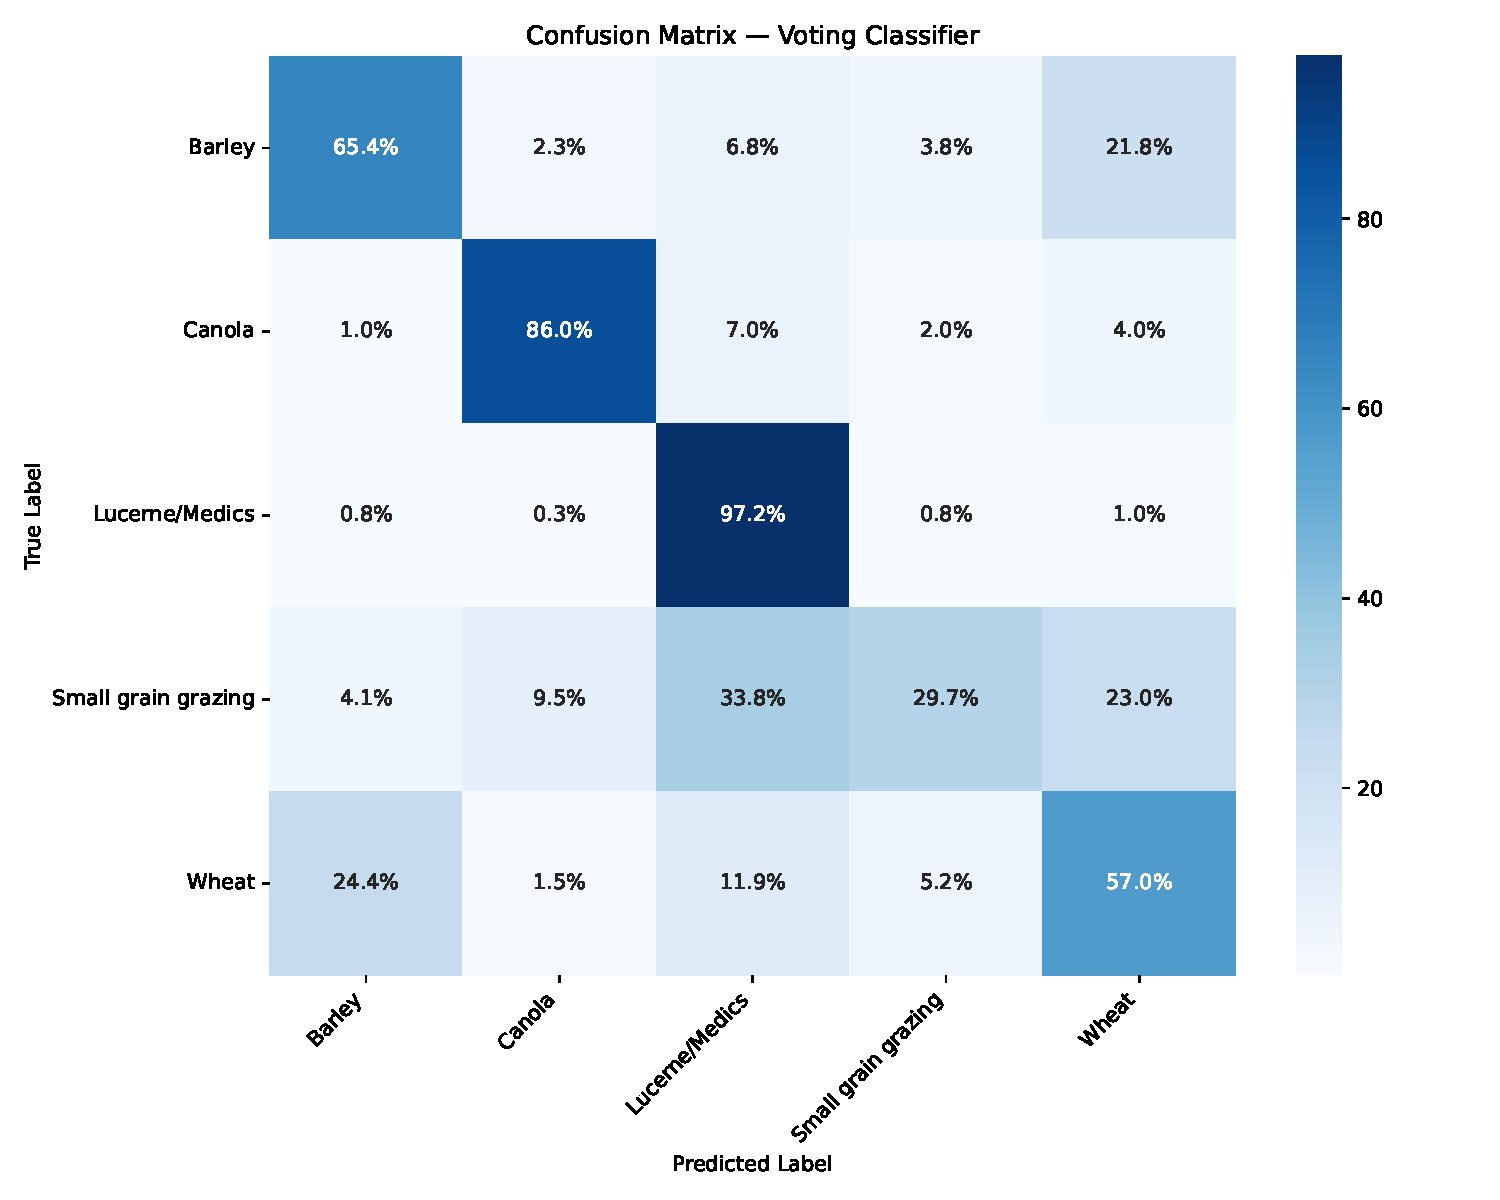
\includegraphics[width=0.55\linewidth]{confusion_matrix_Voting_Classifier.pdf}
\caption{Confusion matrix for the Voting Ensemble at the field level.}
\label{fig:conf_field_voting}
\end{figure}

% ================================================================
\subsection{Deep Learning}
% ================================================================

\subsubsection{Field-Level Results}

Table~\ref{tab:final_results} highlights the benefits of temporal modeling and imbalance-aware training for crop classification. The CNN-BiLSTM with Focal Loss model achieved the highest field-level performance, with a Cohen’s Kappa of 0.77 and an F1 score of 0.84, demonstrating superior ability to capture vegetation dynamics and handle class imbalance.
        
\begin{table}[htbp]
\centering
\caption{Comparison of test-set performance across deep learning models at the field level.
\dag\ denotes the best-performing model.}
\label{tab:final_results}
\renewcommand{\arraystretch}{1.1}
\setlength{\tabcolsep}{6pt}
\begin{tabular}{lccc}
\toprule
\textbf{Model} & \textbf{Kappa} & \textbf{F1} & \textbf{Entropy} \\
\midrule
1D CNN + Optuna                  & 0.69 & 0.78 & 8.03 \\
Ensemble TabNet Classifier         & 0.73 & 0.80 & 6.95 \\
CNN + Bi-LSTM + Focal Loss\textsuperscript{\dag} & 0.77 & 0.84 & 5.91 \\
\bottomrule
\end{tabular}
\end{table}

        The Ensemble TabNet Classifier achieved a field-level Cohen’s Kappa of 0.73 and an F1 score of 0.80, highlighting the strength of attentive feature selection in high-dimensional crop data~\cite{tabnet2024}. Despite lacking explicit temporal modeling, its sequential decision process effectively captured latent phenological patterns. 
        The 1D CNN, while simpler, still delivered competitive results with a Cohen’s Kappa of 0.69 and an F1 score of 0.78, benefiting from Optuna-based hyperparameter optimization[\ref{tab:optuna_top_trials}]. This supports prior observations~\cite{cnn_optuna} that shallow Conv1D architectures, when carefully tuned, can perform strongly for vegetation classification.

            \begin{figure}[htbp]
            \centering
            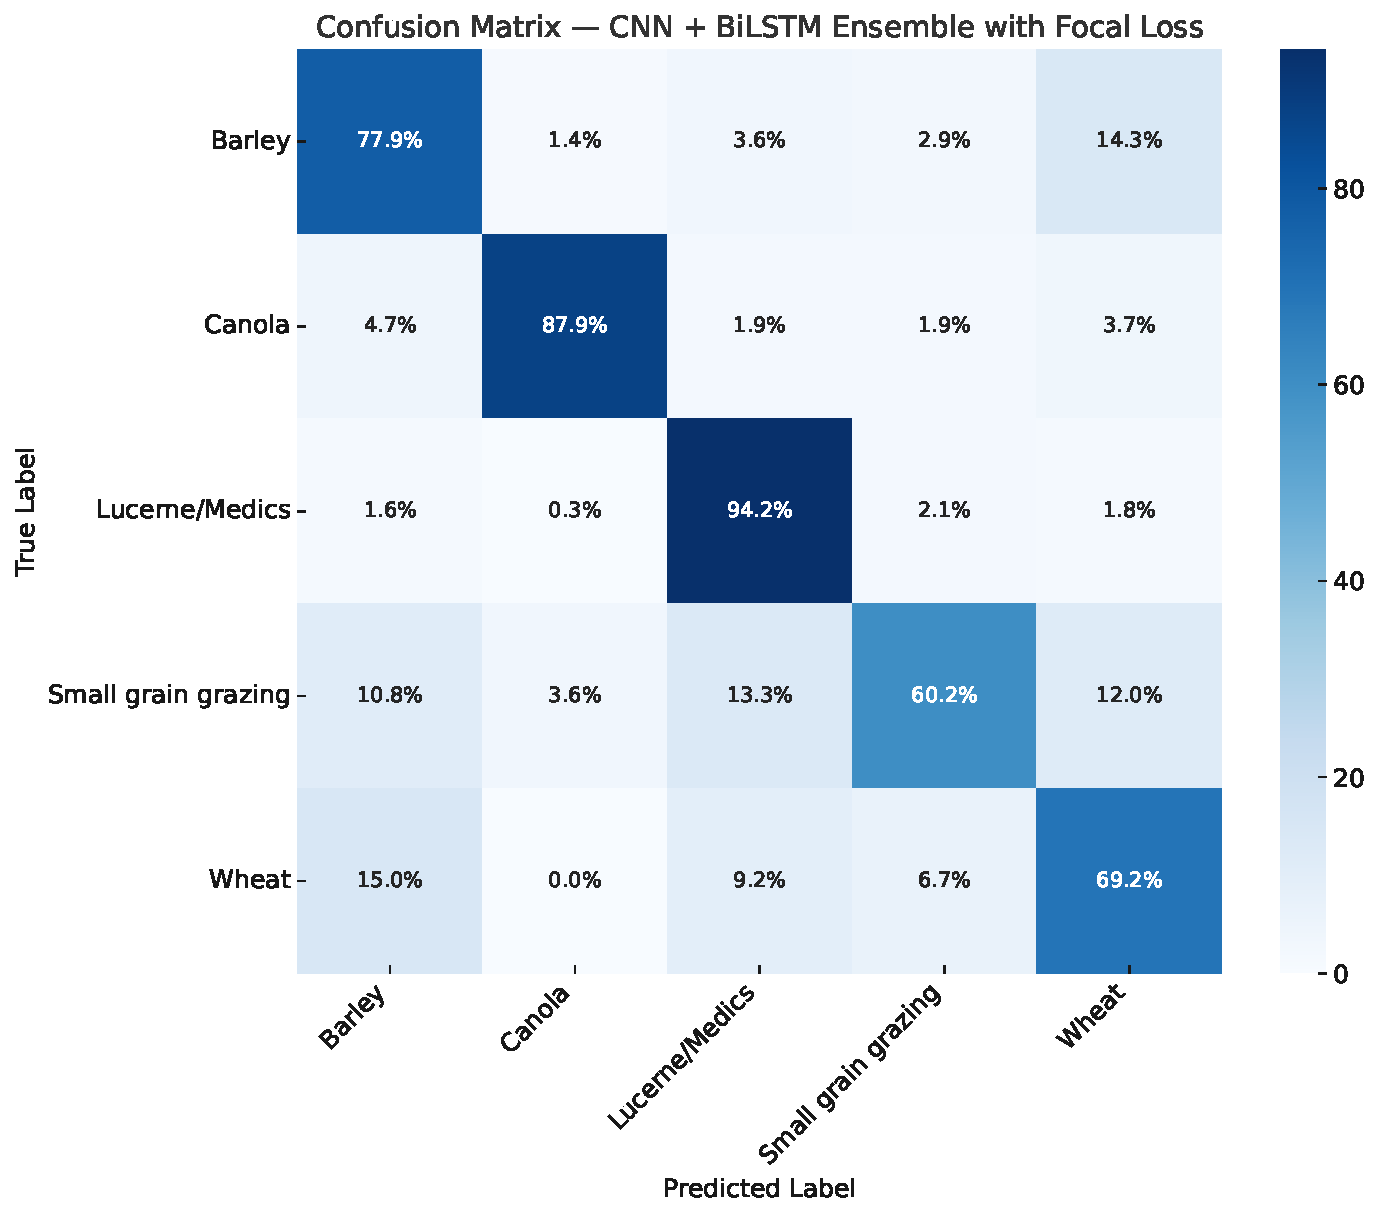
\includegraphics[width=0.45\textwidth]{confusion_matrix_bilstm_percent.pdf}
            \caption{Field-level confusion matrix for CNN + BiLSTM ensemble model showing predicted vs. actual crop classes.}
            \label{fig:conf_matrix_bilstm}
            \end{figure}
            

\subsubsection{Patch-Level Results}

Table~\ref{tab:dl_patch_results} reports performance for the four patch-based
architectures. The 3D CNN Ensemble achieves the highest result (Kappa 0.66,
F1 0.75), marginally ahead of the standalone 3D CNN (Kappa 0.65, F1 0.74).
By modelling volumetric relationships across the spatial and spectral dimensions
jointly, the 3D CNN captures crop-specific texture and phenological trajectories
that the Multi-Channel 2D CNN (Kappa 0.62, F1 0.70) treats independently.
The confusion matrix for the 3D CNN is shown in Figure~\ref{fig:conf_dl_patch};
as with the classical models, small grain grazing (45.9\% correctly classified)
and barley (61.1\%) remain the most difficult classes.

The Transformer-based model performs substantially worse (Kappa 0.48, F1 0.60)
and also has the highest entropy (13.11), indicating less confident predictions.
One contributing factor is the limited spatial inductive bias in the architecture.
In our implementation, each $128 \times 128$ patch is first summarized into a compact
feature vector per time step using a shallow convolutional encoder and global
average pooling, after which self-attention is applied only across the temporal
dimension. While this design enables efficient temporal modeling, it reduces
fine-grained spatial detail within each patch that can be important for
distinguishing spectrally similar crop types.

As a result, the model must learn spatial relationships from aggregated
representations, which is more challenging than in CNN-based patch models that
preserve local spatial context. In addition, the relatively small number of labeled
samples per class at the patch level may further limit the effectiveness of
attention-based learning. Transformer architectures typically benefit from larger
datasets to learn robust feature representations, and in smaller-data settings they
may exhibit reduced generalization or mild overfitting. In our case, this is reflected
in both the lower Kappa score and higher entropy, suggesting that the model struggled
to learn stable, discriminative patterns across crop classes.

This observation is consistent with prior work highlighting the challenges of
generalization in remote sensing deep learning models, particularly when spatial
and spectral structure is not adequately preserved~\cite{pankajakshan2026}.

\begin{table}[htbp]
\centering
\caption{Out-of-sample performance for patch-level deep learning models.
\dag\ denotes the best-performing model at this level.}
\label{tab:dl_patch_results}
\renewcommand{\arraystretch}{1.1}
\setlength{\tabcolsep}{6pt}
\begin{tabular}{lccc}
\toprule
\textbf{Model} & \textbf{Kappa} & \textbf{F1} & \textbf{Entropy} \\
\midrule
Multi-Channel CNN                           & 0.62 & 0.70 & 10.57 \\
3D CNN                                      & 0.65 & 0.74 &  8.99 \\
Transformer-based model                     & 0.48 & 0.60 & 13.11 \\
3D CNN Ensemble\textsuperscript{\dag}       & 0.66 & 0.75 &  8.82 \\
\bottomrule
\end{tabular}
\end{table}

\begin{figure}[htbp]
\centering
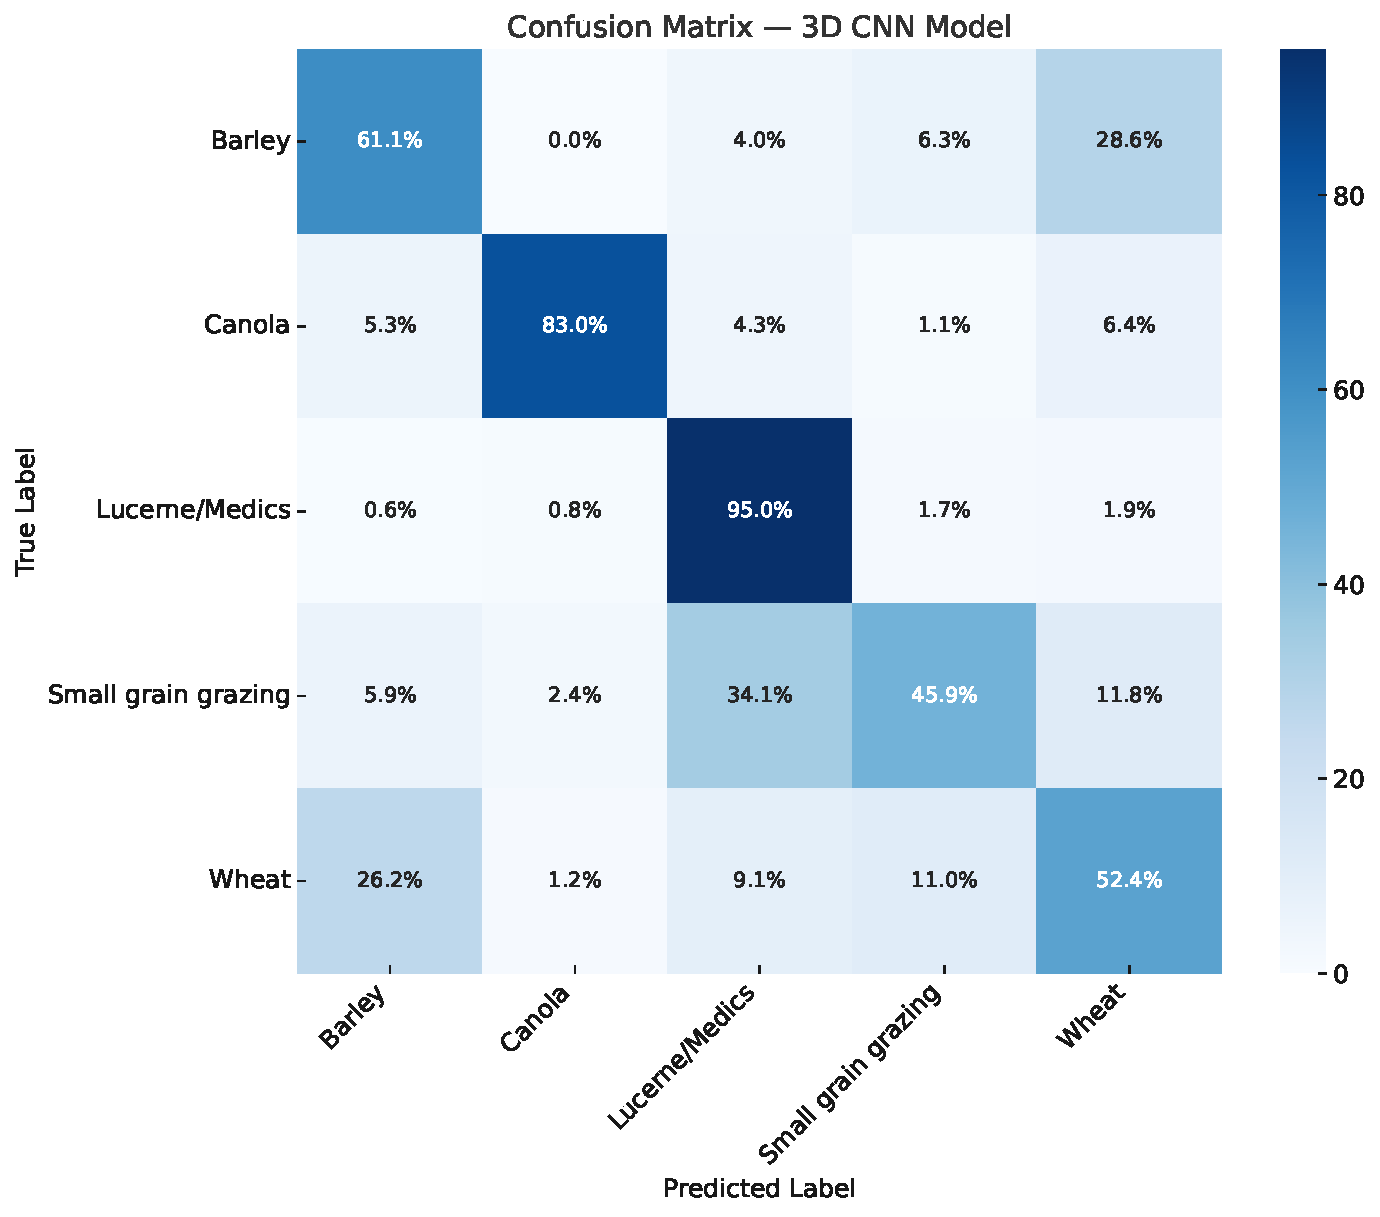
\includegraphics[width=0.55\linewidth]{confusion_matrix_3dcnn.pdf}
\caption{Confusion matrix for the 3D CNN at the patch level.}
\label{fig:conf_dl_patch}
\end{figure}


% ================================================================
\section{Discussion}
% ================================================================

Our results demonstrate that the choice of modeling paradigm involves meaningful
trade-offs between predictive performance, computational cost, and interpretability, with no single approach dominating across all criteria.

\paragraph{Deep learning and temporal sequence modeling.}

The CNN-BiLSTM ensemble achieved the strongest field-level performance (Kappa
0.77, F1 0.84), outperforming the best classical approach by approximately 0.08
in both metrics. This advantage is consistent with findings by Bandar and
Co\c{s}kuncay~\cite{bandar2024bilstm}, who reported an F1 of 0.82 and Kappa of 0.76
using a comparable Bi-LSTM attention hybrid on the BreizhCrop dataset, and with
Tufail et al.~\cite{tufail2025cnnrnn}, who demonstrated that CNN-RNN hybrids
outperform purely temporal or spatial models for spectrally similar crops in
Northern Italy. The margin of improvement observed here suggests that direct
sequence modeling over raw reflectance values captures phenological dynamics
that even rich automated feature sets partially miss. The use of Focal Loss and
weighted sampling appears important in this context: without explicit
imbalance mitigation, the model would likely default toward lucerne/medics, the
dominant class, at the expense of rarer classes.

\paragraph{Classical machine learning and automated feature extraction.}

Despite the deep learning advantage, the field-level Voting Classifier (Kappa
0.69, F1 0.76) outperformed several individual deep learning architectures,
including TabNet and the 1D CNN, at substantially lower computational cost. This
is consistent with the broader literature suggesting that well-tuned ensemble
classifiers with rich temporal features remain competitive in crop classification
tasks~\cite{mann2025, mahlayeye2024}. The use of \texttt{xr\_fresh} for
automated feature extraction is a key factor here: rather than relying on a
small set of manually chosen indices, the framework produces a comprehensive
set of statistical and temporal descriptors that partially approximate what
sequence models learn implicitly. To our knowledge this is the first evaluation
of \texttt{xr\_fresh} in a crop classification context, and these results
suggest it is a viable alternative to hand-crafted feature pipelines.

\paragraph{Patch-level spatial modeling.}

Patch-level 3D CNN models (Kappa 0.66, F1 0.75) matched classical model
performance but did not exceed it or the CNN-BiLSTM. This is partly expected:
at Sentinel-2's 10–20 m resolution, individual fields in the Western Cape are
often small enough that a 100×100 pixel patch covers multiple fields or
includes substantial mixed-boundary pixels, introducing label noise. The fixed
grid placement compounds this by omitting boundary pixels entirely. The 3D CNN
still outperformed the 2D multi-channel CNN, confirming that joint
spatiotemporal convolution adds discriminative value over treating temporal
observations as independent channels. The Transformer-based model performed
substantially worse (Kappa 0.48), consistent with evidence that attention-based
architectures without convolutional inductive biases require pre-training or
large domain-specific datasets to be competitive~\cite{pankajakshan2026}.

\paragraph{Persistent difficulty with small grain grazing and barley.}

Small grain grazing is the most consistently misclassified crop across all
models and paradigms — even the best-performing CNN-BiLSTM struggles with it.
This is not surprising given the class has the fewest training fields
(Figure~\ref{fig:EDA-1}) and its spectral-temporal signature closely
resembles barley and wheat, particularly during early growth stages. The
confusion between barley and wheat is similarly persistent across all methods.
These two failure modes likely share a common cause: insufficient within-class
phenological diversity in the training data to allow models to learn
discriminative boundaries. No amount of architectural sophistication fully
compensates for this. Future data collection efforts in this region should
specifically target these minority classes.

\paragraph{Limitations.}

Several limitations constrain the interpretation of these results. First, all
experiments use a single growing season (2017) from a single region, limiting
conclusions about temporal and geographic generalizability. Second, the
\texttt{xr\_fresh} feature set of 174 dimensions per pixel was used without
formal feature selection, and it is likely that many features are correlated or
weakly informative. Dimensionality reduction or feature importance analysis
could reduce training complexity and potentially improve generalization. Third,
the exclusion of SAR data, while methodologically motivated, limits the ceiling
performance achievable, particularly for crops with similar optical signatures.
Finally, EVI was computed from monthly median composites rather than
simultaneous band acquisitions, which may introduce spectral inconsistencies.

% ================================================================
\section{Conclusion}
% ================================================================

This study provides a systematic evaluation of crop classification methods using multi-temporal Sentinel-2 optical imagery in the Western Cape of South Africa — a region that combines the environmental complexity typical of Global South dryland farming with an unusually rich labeled dataset, making it well suited for rigorous inter-paradigm comparison.

The CNN-BiLSTM ensemble achieved the strongest field-level results (F1 0.84, Kappa 0.77), demonstrating that end-to-end sequence modeling over raw spectral time series can outperform automated feature engineering pipelines in complex agricultural landscapes. Classical ensemble methods paired with \texttt{xr\_fresh} feature extraction remained competitive at substantially lower computational cost, with the field-level Voting Classifier achieving Kappa 0.69 and F1 0.76 — making classical approaches a practical choice in resource-constrained or operational settings where interpretability and deployment speed matter. Patch-based 3D CNN models contributed spatial context but did not surpass pixel-level deep learning, partly due to field size and boundary effects at Sentinel-2's native resolution.

Across all models, small grain grazing and barley-wheat confusion represent persistent challenges that architectural choices alone cannot resolve. Addressing these will require either richer temporal sampling — for instance, using all available Sentinel-2 acquisitions rather than monthly composites — or targeted data collection for underrepresented classes.

Looking ahead, the most productive directions for this setting are multi-source data fusion incorporating SAR imagery, domain adaptation to extend models across growing seasons and regions, and hybrid workflows that combine \texttt{xr\_fresh} feature richness with patch-based spatial representations. Higher-cadence optical platforms such as PlanetScope could substantially mitigate the cloud cover and temporal resolution limitations that constrained this study, and provide a path toward operational crop monitoring systems scalable to national or continental extents.

\section*{Conflict of Interest}

The authors declare that they have no competing interests.

\section*{Data Availability}

This study relied on multiple sources of data. Ground-truth crop type labels were obtained from Radiant Earth’s MLHub platform \cite{mlhub}, while multi-temporal Sentinel-2 imagery was extracted using the Google Earth Engine API. Since the raw data was processed and combined in various ways specific to this study, the resulting dataset used for model training and evaluation is not hosted publicly but can be shared by the authors upon reasonable request for academic or research purposes.

\section*{Code Availability}

All source code used for data processing, modeling, and evaluation is publicly available \cite{capstone_repo}.

\bibliographystyle{sn-mathphys} % Use Springer Nature's preferred style
\begin{thebibliography}{99}


\bibitem{sciencedirect2023}
Ali S, Usama M, Usman M, Rizwan M, Rehman A (2023) A hybrid deep learning model for crop classification using Sentinel-2 time series data. \textit{Comput Electron Agric} 206:107673.

\bibitem{ieee2017}
Ienco D, Gaetano R, Dupaquier C, Maurel P (2017) Land cover classification via 
multitemporal spatial data by recurrent neural networks. \textit{arXiv preprint} 
arXiv:1704.04055. \href{https://arxiv.org/abs/1704.04055}{paper}

\bibitem{mlhub}
Radiant Earth Foundation (2024) South Africa Crop Type Competition. Source Cooperative repository.

\bibitem{capstone_repo}
Capstone Group 3 (2025) Capstone\_Group\_3: Source code for multitemporal crop classification. \textit{GitHub repository}
\href{https://github.com/DishaKacha7/Capstone_Group_3}{Github}

\bibitem{sar2022}
Kordi F, Yousefi H (2022) Crop classification based on phenology information using time series of optical and synthetic-aperture radar images. \textit{Remote Sens Appl Soc Environ} 27:100812.


\bibitem{fan2023hcrnn}
Fan X, Chen L, Xu X, Yan C, Fan J, Li X (2023) Land Cover Classification of Remote Sensing Images Based on Hierarchical Convolutional Recurrent Neural Network. Forests 14(9):1881. https://doi.org/10.3390/f14091881

\bibitem{tufail2025cnnrnn}
Tufail R, Tassinari P, Torreggiani D (2025) Deep Learning Applications for Crop Mapping Using Multi-Temporal Sentinel-2 Data and Red-Edge Vegetation Indices: Integrating Convolutional and Recurrent Neural Networks. Remote Sens 17(18):3207. https://doi.org/10.3390/rs17183207

\bibitem{bandar2024bilstm}
Bandar A, Co\c{s}kun\c{c}ay A (2024) Crop Classification with Attention Based BI-LSTM and Temporal Convolution Neural Network Combination for Remote Sensing BreizhCrop Time Series Data. Y\"uz\"unc\"u Y{\i}l \"Universitesi Fen Bilimleri Enstit\"us\"u Dergisi 29(1):173--188. https://doi.org/10.53433/yyufbed.1335866

\bibitem{mann2023}
Mann ML, Colson L, Nealon R, Engstrom R, Nakacwa S (2023) Lite Learning: Efficient Crop Classification in Tanzania Using Traditional Machine Learning \& Crowd Sourcing. \textit{SSRN Preprint}.

\bibitem{medium2023}
Chauhan A (2023) Crop Classification via Satellite Image Time Series and PSETAE Deep Learning Model. \textit{Medium}.

\bibitem{feyisa2020}
Feyisa GL, Palao LK, Nelson A, Gumma MK, Paliwal A, Win KT, Nge KH, Johnson DE (2020) Characterizing and mapping cropping patterns in a complex agro-ecosystem: an iterative participatory mapping procedure using machine learning algorithms and MODIS vegetation indices. \textit{Comput Electron Agric} 175:105595. \href{https://doi.org/10.1016/j.compag.2020.105595}{https://doi.org/10.1016/j.compag.2020.105595}

\bibitem{saini2018}
Saini R, Ghosh SK (2018) Crop classification on single date Sentinel-2 imagery using random forest and support vector machine. \textit{Int Arch Photogramm Remote Sens Spatial Inf Sci} XLII-5:683--688. \href{https://doi.org/10.5194/isprs-archives-xlii-5-683-2018}{https://doi.org/10.5194/isprs-archives-xlii-5-683-2018}

\bibitem{jin2019}
Jin Z, Azzari G, You C, Di Tommaso S, Aston S, Burke M, Lobell DB (2019) Smallholder maize area and yield mapping at national scales with Google Earth Engine. \textit{Remote Sens Environ} 228:115--128. \href{https://doi.org/10.1016/j.rse.2019.04.016}{https://doi.org/10.1016/j.rse.2019.04.016}

\bibitem{penabarragan2011}
Pe\~na-Barrag\'an JM, Ngugi MK, Plant RE, Six J (2011) Object-based crop identification using multiple vegetation indices, textural features and crop phenology. \textit{Remote Sens Environ} 115:1301--1316. \href{https://doi.org/10.1016/J.RSE.2011.01.009}{https://doi.org/10.1016/J.RSE.2011.01.009}

\bibitem{belgiu2016}
Belgiu M, Dr\u{a}gu\c{t} L (2016) Random forest in remote sensing: A review of applications and future directions. \textit{ISPRS J Photogramm Remote Sens} 114:24--31. \href{https://doi.org/10.1016/j.isprsjprs.2016.01.011}{https://doi.org/10.1016/j.isprsjprs.2016.01.011}

\bibitem{kuwait2023}
Rangarajan AK, Purushothaman R, Prabhakar M, Szczepanski C (2023) Crop identification and disease classification using traditional machine learning and deep learning approaches. \textit{J Eng Res} 11(1B):1--12.

\bibitem{acm2020}
Gadiraju KK, Ramachandra B, Chen Z, Vatsavai RR (2020) Weakly supervised deep learning for rapid crop cover mapping with multi-temporal satellite imagery. In: \textit{Proc 26th ACM SIGKDD Int Conf Knowl Discov Data Min}.

\bibitem{liu2022}
Liu X, et al. (2022) Deep learning for crop classification. \textit{IEEE Trans Geosci Remote Sens} 60:1--14.

\bibitem{russwurm2018}
Russwurm M, Koerner M (2018) Temporal CNN for crop analysis. \textit{Remote Sens} 10(12):1930.

\bibitem{sa_comp}
Radiant Earth (2024) Spot The Crop Challenge. \href{https://github.com/radiantearth/spot-the-crop-challenge}{GitHub repository}.

\bibitem{campbell2011introduction}
Campbell JB, Wynne RH (2011) \textit{Introduction to Remote Sensing}. Guilford Press.
 
\bibitem{wardlow2007towards}
Wardlow BD, Melendez SN, Justice CM (2007) Towards an operational system for cropland monitoring using MODIS time series data. \textit{Remote Sens Environ} 110(3):349--361.

\bibitem{james2013}
James G, Witten D, Hastie T, Tibshirani R (2013) \textit{An Introduction to Statistical Learning}. Springer.

\bibitem{breiman2001}
Breiman L (2001) Random forests. \textit{Machine Learning} 45(1):5--32.


\bibitem{ke2017}
Ke G, Meng Q, Finley T, et al. (2017) LightGBM: A highly efficient gradient boosting decision tree. \textit{NeurIPS} 30.

\bibitem{chen2016}
Chen T, Guestrin C (2016) XGBoost: A scalable tree boosting system. In: \textit{Proc 22nd ACM SIGKDD Int Conf Knowl Discov Data Min}, pp 785--794.

\bibitem{friedman2001}
Friedman JH (2001) Greedy function approximation: A gradient boosting machine. \textit{Ann Stat} 29(5):1189--1232.

\bibitem{maxwell2019}
Maxwell AE, Warner TA, Fang F (2019) Implementation of machine-learning classification in remote sensing: an overview. \textit{Remote Sens} 11(14):1633.

\bibitem{zhu2017}
Zhu XX, Tuia D, Mou L, et al. (2017) Deep learning in remote sensing: A comprehensive review and list of resources. \textit{IEEE Geosci Remote Sens Mag} 5(4):8--36.

\bibitem{li2019}
Li R, Zheng S, Zhang C, Huang C (2019) Object detection in remote sensing images based on improved Faster R-CNN. \textit{IEEE Access} 7:35813--35822.


\bibitem{cnn_multitemp}
Kussul N, Lavreniuk M, Skakun S, Shelestov A (2017) Deep Learning Classification of Land Cover and Crop Types Using Remote Sensing Data. \textit{IEEE Geosci Remote Sens Lett} 14(5):778--782.

\bibitem{tabnet2024}
Muruganantham P, Wibowo S, Grandhi S, Islam N (2024) A Deep Learning Approach for Dealing with Tabular Data in Crop Classification. \textit{Proc IEEE Int Conf ICT Convergence (ICTC)}:2054--2059. doi:10.1109/ICTC62082.2024.10826760

\bibitem{cnn_optuna}
Zhong L, Hu L, Zhou H (2018) Deep learning based multi-temporal crop classification. \textit{Remote Sens Environ} 221:430--443. doi:10.1016/j.rse.2018.11.032

\bibitem{rustowicz2019}
Rustowicz RM, Singh A, Davis A (2019) Semantic segmentation of crop type in African smallholder agriculture. In: \textit{Proc IEEE/CVF CVPR Workshops}, pp 75--82.


\bibitem{cropformer2023}
Zhao Y, Li W, Li M, Wang J (2023) Cropformer: A new generalized deep learning classification framework for multi-scenario crop classification. \textit{Front Plant Sci} 14:1130659.


\bibitem{mahlayeye2024}
Mahlayeye M, Darvishzadeh R, Nelson A (2024) Characterising maize and intercropped maize spectral signatures for cropping pattern classification. \textit{Int J Appl Earth Obs Geoinf} 128:103699.


\bibitem{mann2017}
Mann ML, Warner JM (2017) Ethiopian wheat yield and yield gap estimation: A spatially explicit small area integrated data approach. \textit{Field Crops Res} 201:60--74.

\bibitem{mann2019}
Mann ML, Warner JM, Malik AS (2019) Predicting high-magnitude, low-frequency crop losses using machine learning: an application to cereal crops in Ethiopia. \textit{Clim Change} 154:211--227.

\bibitem{mann2025}
Mann ML (2025) xr\_fresh: Automated Time Series Feature Extraction for Remote Sensing and Gridded Data. \textit{J Open Source Softw} 10(115):9009.

\bibitem{teixeira2023}
Teixeira I, Morais R, Sousa JJ, Cunha A (2023) Deep Learning Models for the Classification of Crops in Aerial Imagery: A Review. \textit{Agriculture} 13(5):965.

\bibitem{hohl2024}
Höhl A, Obadic I, Fernández-Torres MÁ, Oliveira D, Zhu XX (2024) Recent Trends Challenges and Limitations of Explainable AI in Remote Sensing. In: \textit{Proc IEEE/CVF Conf Comput Vis Pattern Recognit}, pp 8199--8205.

\bibitem{buttar2024}
Buttar PK et al. (2024) Satellite imagery analysis for crop type segmentation using U-net architecture. \textit{Procedia Comput Sci} 235:3418--3427.

\bibitem{liu2024}
Liu N, Zhao Q, Williams R, Barrett B (2024) Enhanced crop classification through integrated optical and SAR data: a deep learning approach for multi-source image fusion. \textit{Int J Remote Sens} 45(19--20):7605--7633.

\bibitem{pankajakshan2026}
Pankajakshan P, Padmasanan A, Sundar S (2026) Deep Architectures Fail to Generalize: A Lightweight Alternative for Agricultural Domain Transfer in Hyperspectral Images. \textit{Sensors} 26(1):174.

\bibitem{espejo2020}
Espejo-Garcia B, Mylonas N, Athanasakos L, Fountas S, Vasilakoglou I (2020) Towards weeds identification assistance through transfer learning. \textit{Comput Electron Agric} 171:105306.

\bibitem{koklu2022}
Koklu M, Unlersen MF, Ozkan IA, Aslan MF, Sabanci K (2022) A CNN-SVM study based on selected deep features for grapevine leaves classification. \textit{Measurement} 188:110425.

\bibitem{yang2020}
Yang S, Gu L, Li X, Jiang T, Ren R (2020) Crop Classification Method Based on Optimal Feature Selection and Hybrid CNN-RF Networks for Multi-Temporal Remote Sensing Imagery. \textit{Remote Sens} 12(19):3119.

\bibitem{nowakowski2021}
Nowakowski A, Mrziglod J, Spiller D, Bonifacio R, Ferrari I, Mathieu PP, Garcia-Herranz M, Kim DH (2021) Crop type mapping by using transfer learning. \textit{Int J Appl Earth Obs Geoinf} 98:102313.

\bibitem{begue2020}
Bégué, A., Leroux, L., Soumaré, M., Faure, J.F., Diouf, A.A., Augusseau, X., Touré, L., Tonneau, J.P., 2020. Remote sensing products and services in support of agricultural public policies in Africa: overview and challenges. \textit{Frontiers in Sustainable Food Systems}, 4. \href{https://doi.org/10.3389/fsufs.2020.00058}{https://doi.org/10.3389/fsufs.2020.00058}

\end{thebibliography}


\end{document}